\documentclass[aspectratio=169]{beamer}
%\usetheme{Boadilla}
%\usetheme{default}
\usecolortheme{owl}
\usepackage{color}

\usepackage{hyperref}
\hypersetup{
    colorlinks=true,
    linkcolor=blue,
    filecolor=magenta,      
    urlcolor=blue,
}

\urlstyle{same}


\title{You've Been Hacked}
\subtitle{An (Interactive) Course on Web Security}
\author{Paul Duplys}
\institute[]{@duplys}
\date{\today}

\begin{document}

\begin{frame}
    \titlepage
\end{frame}

\begin{frame}
    %\frametitle{Outline}
    \tableofcontents
\end{frame}

\section{0x0: Preliminaries}

{
\usebackgroundtemplate{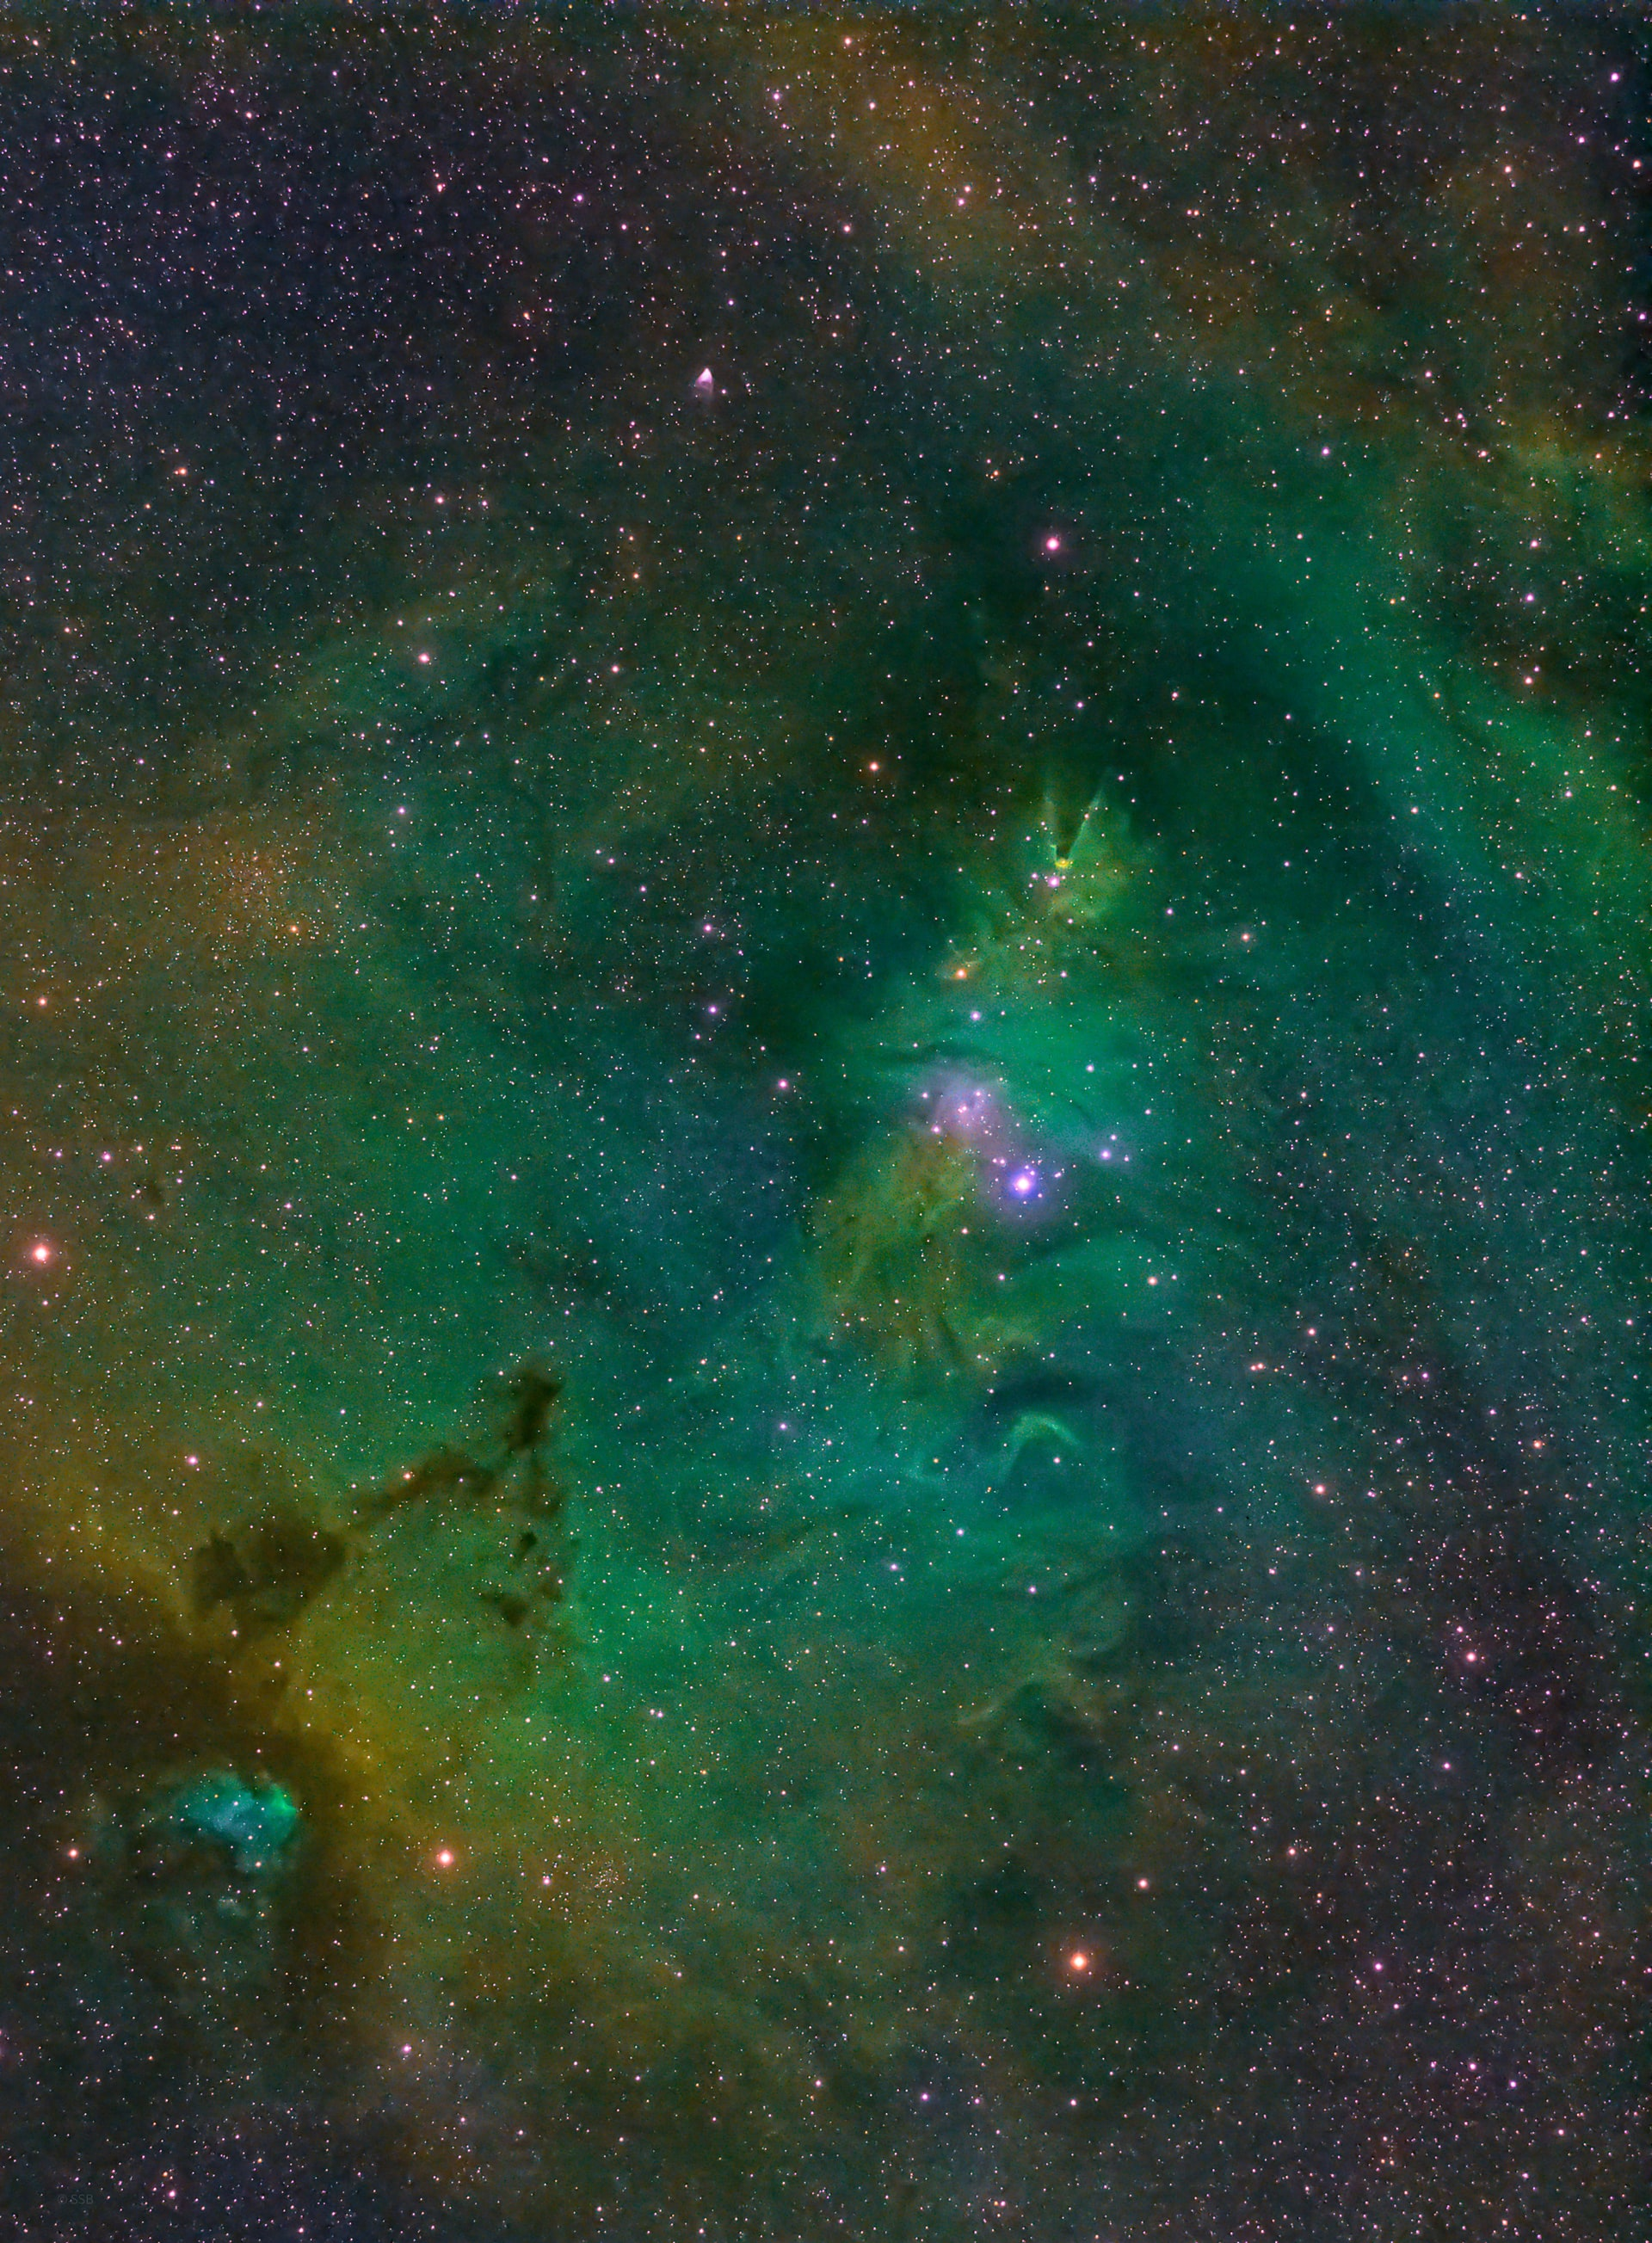
\includegraphics[width=\paperwidth]{./img/aldebaran.jpg}}
\begin{frame}
\huge{\textcolor{white}{\textbf{0x0: Preliminaries}}}
\end{frame}
}

\begin{frame}
    \frametitle{\texttt{whoami}}
    short intro/bio.
\end{frame}

\begin{frame}
    \frametitle{\texttt{man slides}}

    (Interactive) course on web security based on Carsten Eiler's book "You've Been Hacked".
    
    Who is the audience? How can I use the book? How can I explore the app?
\end{frame}

\begin{frame}
    \frametitle{...}
    Where are the instruction located for how to build the Docker files and use the repository?
\end{frame}

\section{0x1: Web Security 101}

{
\usebackgroundtemplate{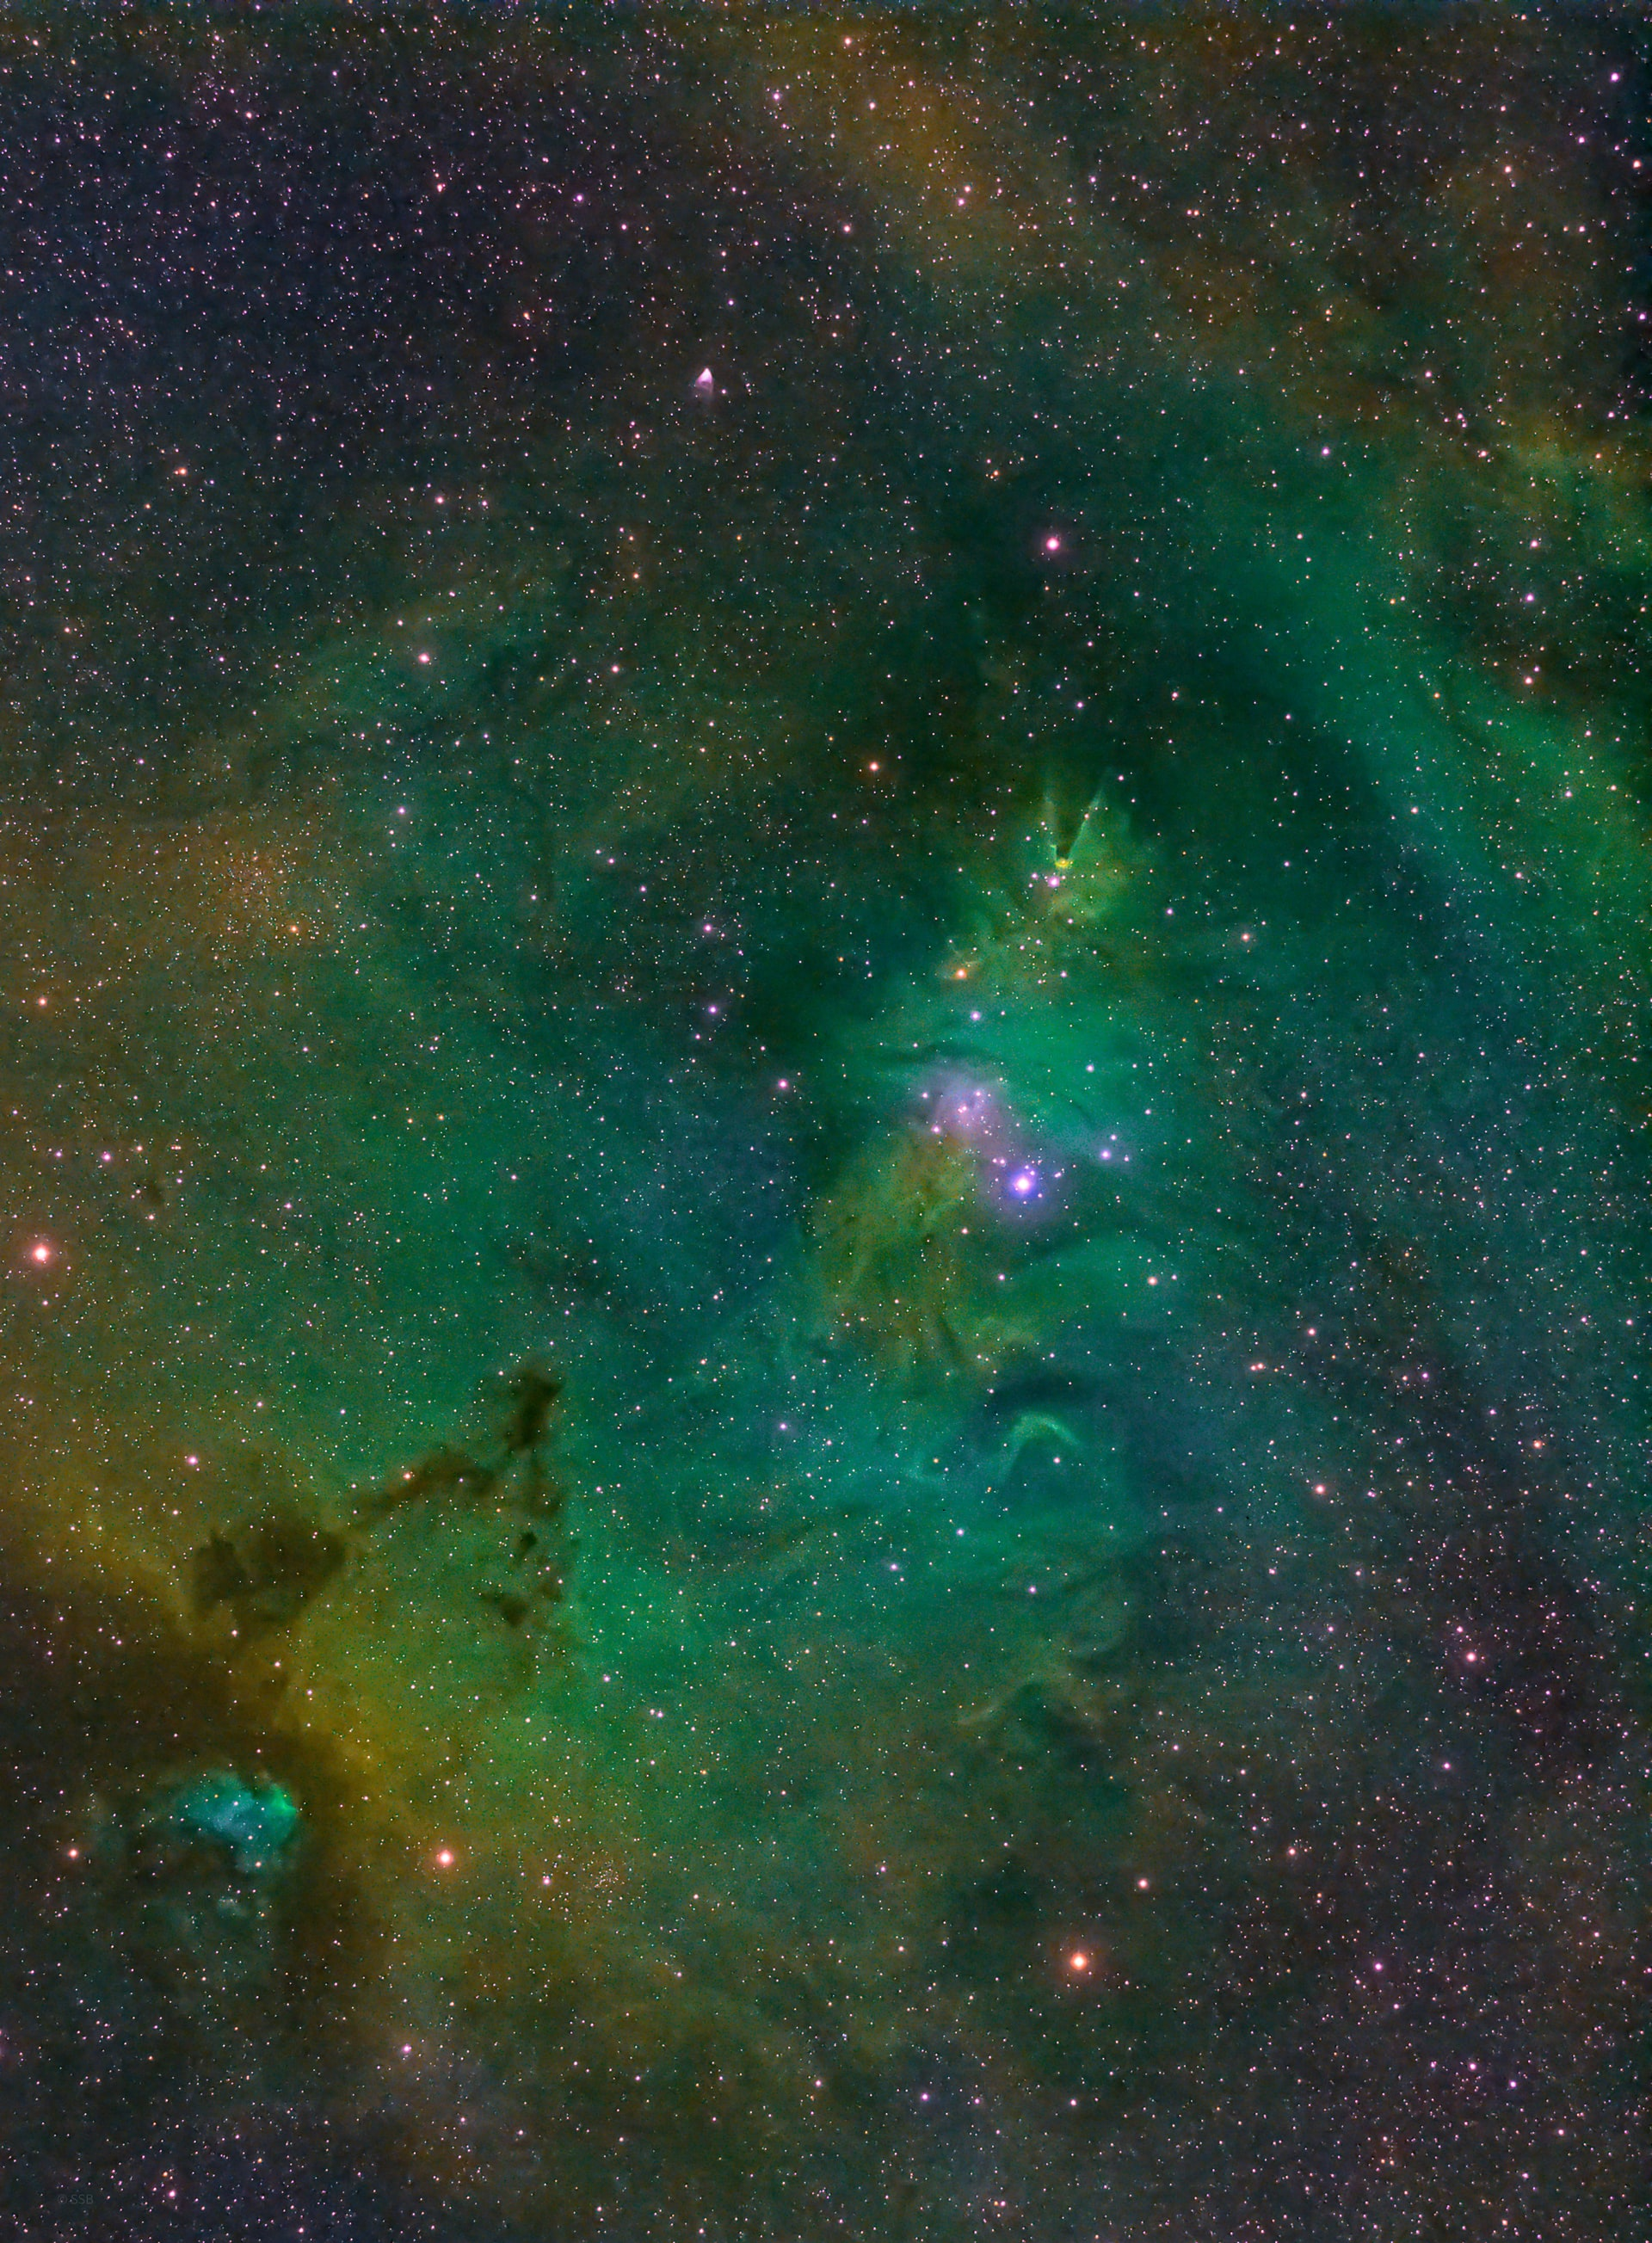
\includegraphics[width=\paperwidth]{./img/aldebaran.jpg}}
\begin{frame}
\huge{\textcolor{white}{\textbf{0x1: Web Security 101}}}
\end{frame}
}

\begin{frame}
    %\frametitle{How Do You Find Vulnerabilities in Web Applications?}
    In a nutshell, \textbf{to find vulnerabilities in your web application}, ...
    \begin{enumerate}
        \item ... test various values for parameters used by the web application and see what happens (conceptually similar to fuzzing)
        \item ... check web application code for bugs that may lead to security vulnerabilities (typically missing checks of input values or missing countermeasures against certain types of attacks)
    \end{enumerate}
\end{frame}

\begin{frame}
    %\frametitle{OWASP TOP 10}

    The \href{https://owasp.org/www-project-top-ten/}{Open Web Application Security Project (OWASP)} maintains a list of Top 10 vulnerabilities in web applications.

    \begin{center}
        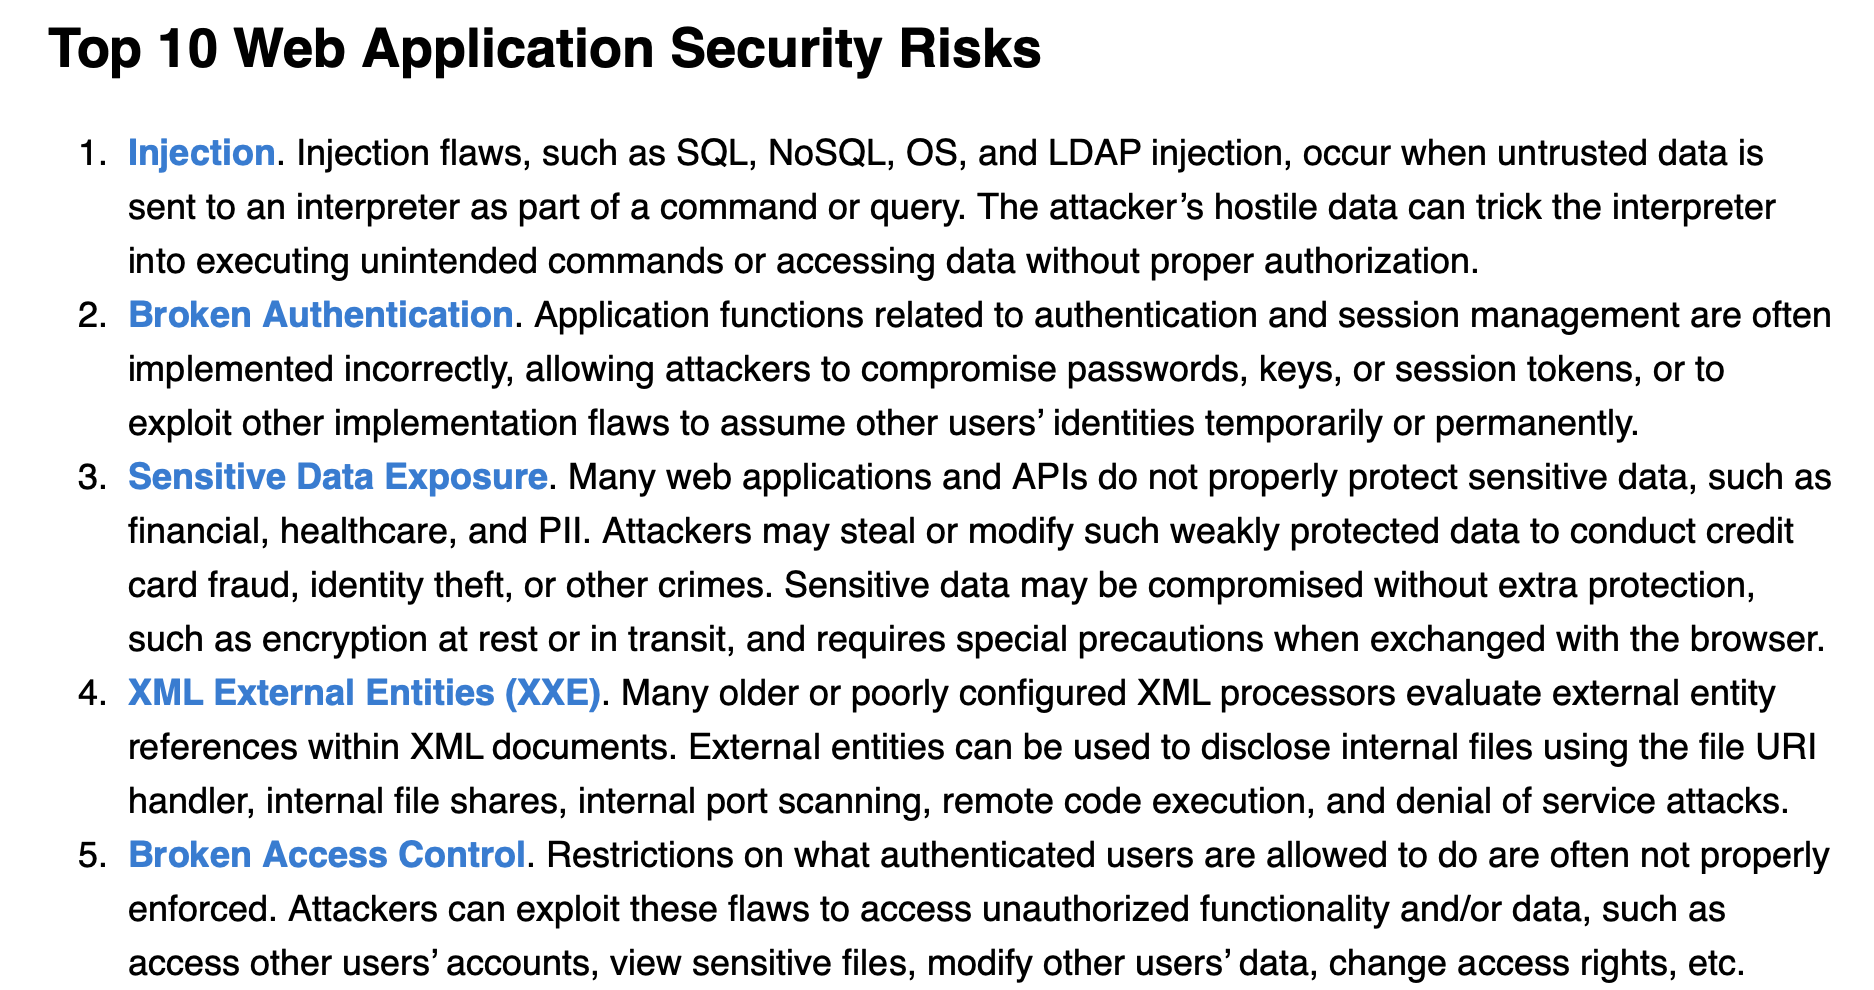
\includegraphics[scale=.35,angle=2]{img/owasp-top10.png}    
    \end{center}
\end{frame}

\begin{frame}
    \frametitle{Fahrplan}

    \begin{itemize}
        \item Get to know your target
        \item Test for stateful attacks
        \item Test for attacks on authentication
        \item Test for cross-site-scripting (XSS)
        \item Test for SQL injection
        \item Test for other injection-based vulnerabilities
        \item Test for attacks on file operations
        \item Test for buffer overflows, format strings and integer bugs
        \item Test for architectural attacks
        \item Test for attacks on the web server 
    \end{itemize}

\end{frame}

\section{0x2: Recon}

{
%\setbeamercolor{background canvas}{bg=yellow}
\usebackgroundtemplate{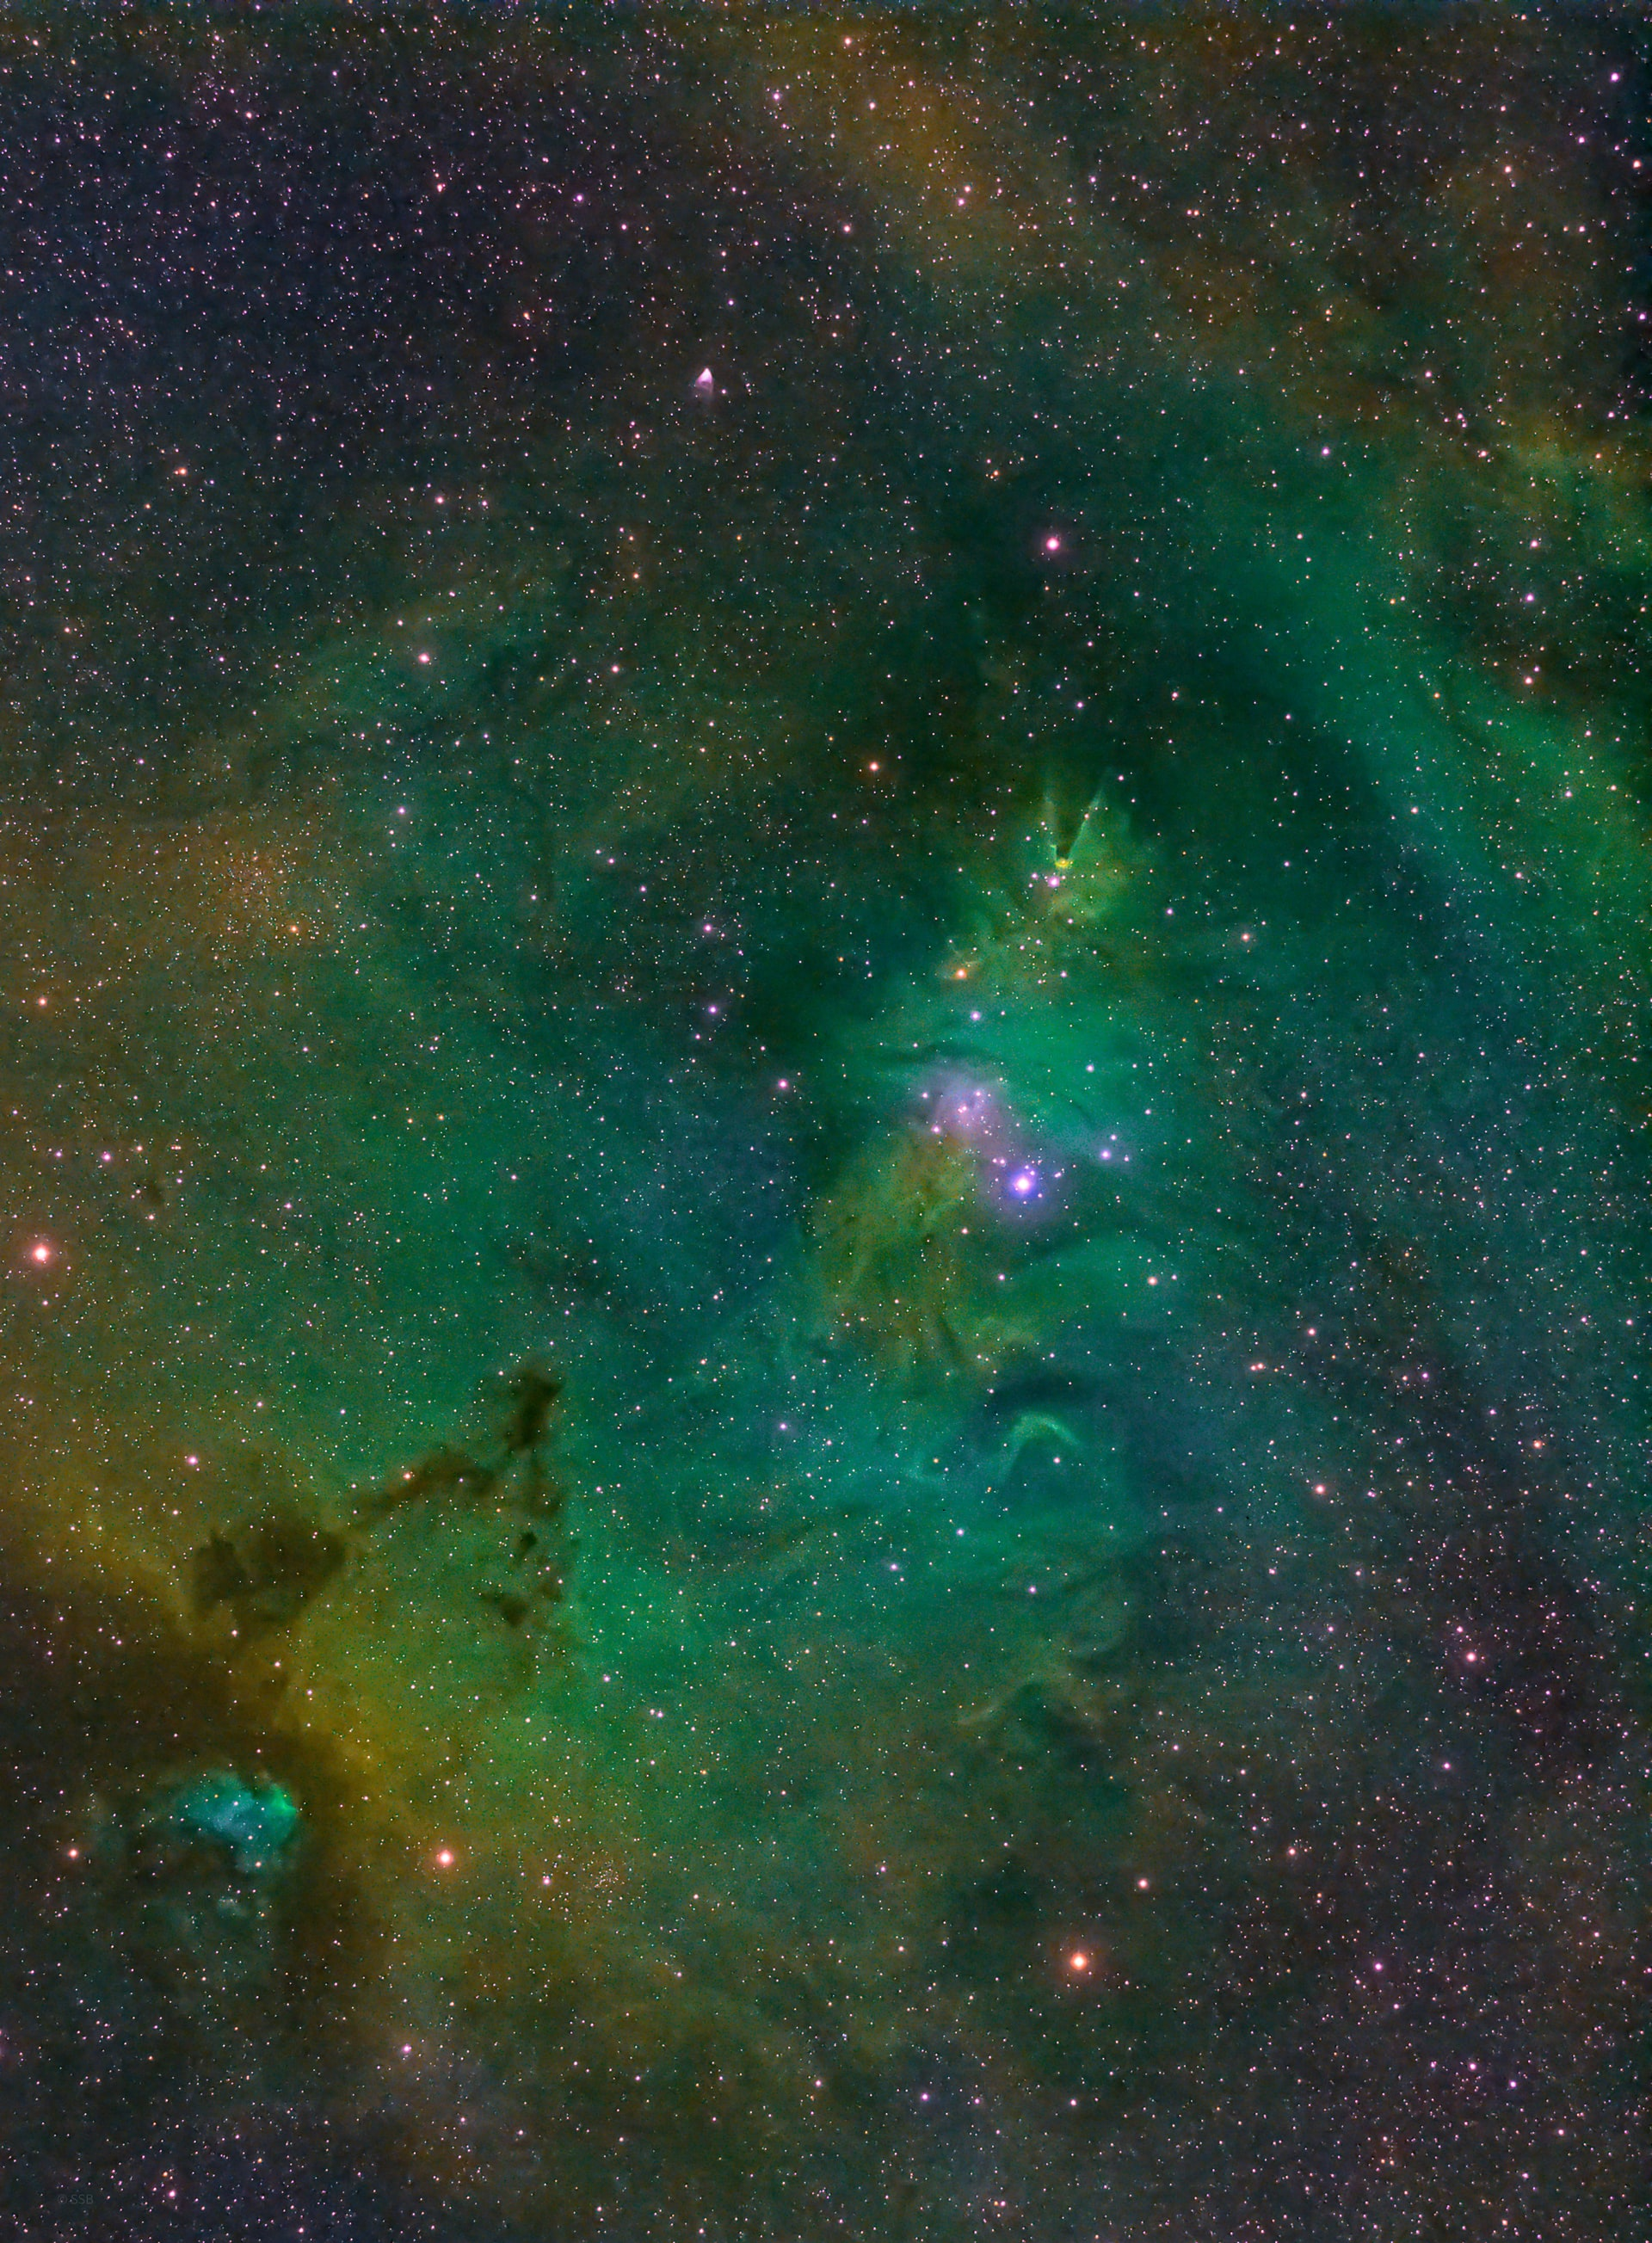
\includegraphics[width=\paperwidth]{./img/aldebaran.jpg}}
\begin{frame}
%\hspace{0.0cm}
\huge{\textcolor{white}{\textbf{0x2: Recon}}}
\end{frame}
}

%\usebackgroundtemplate{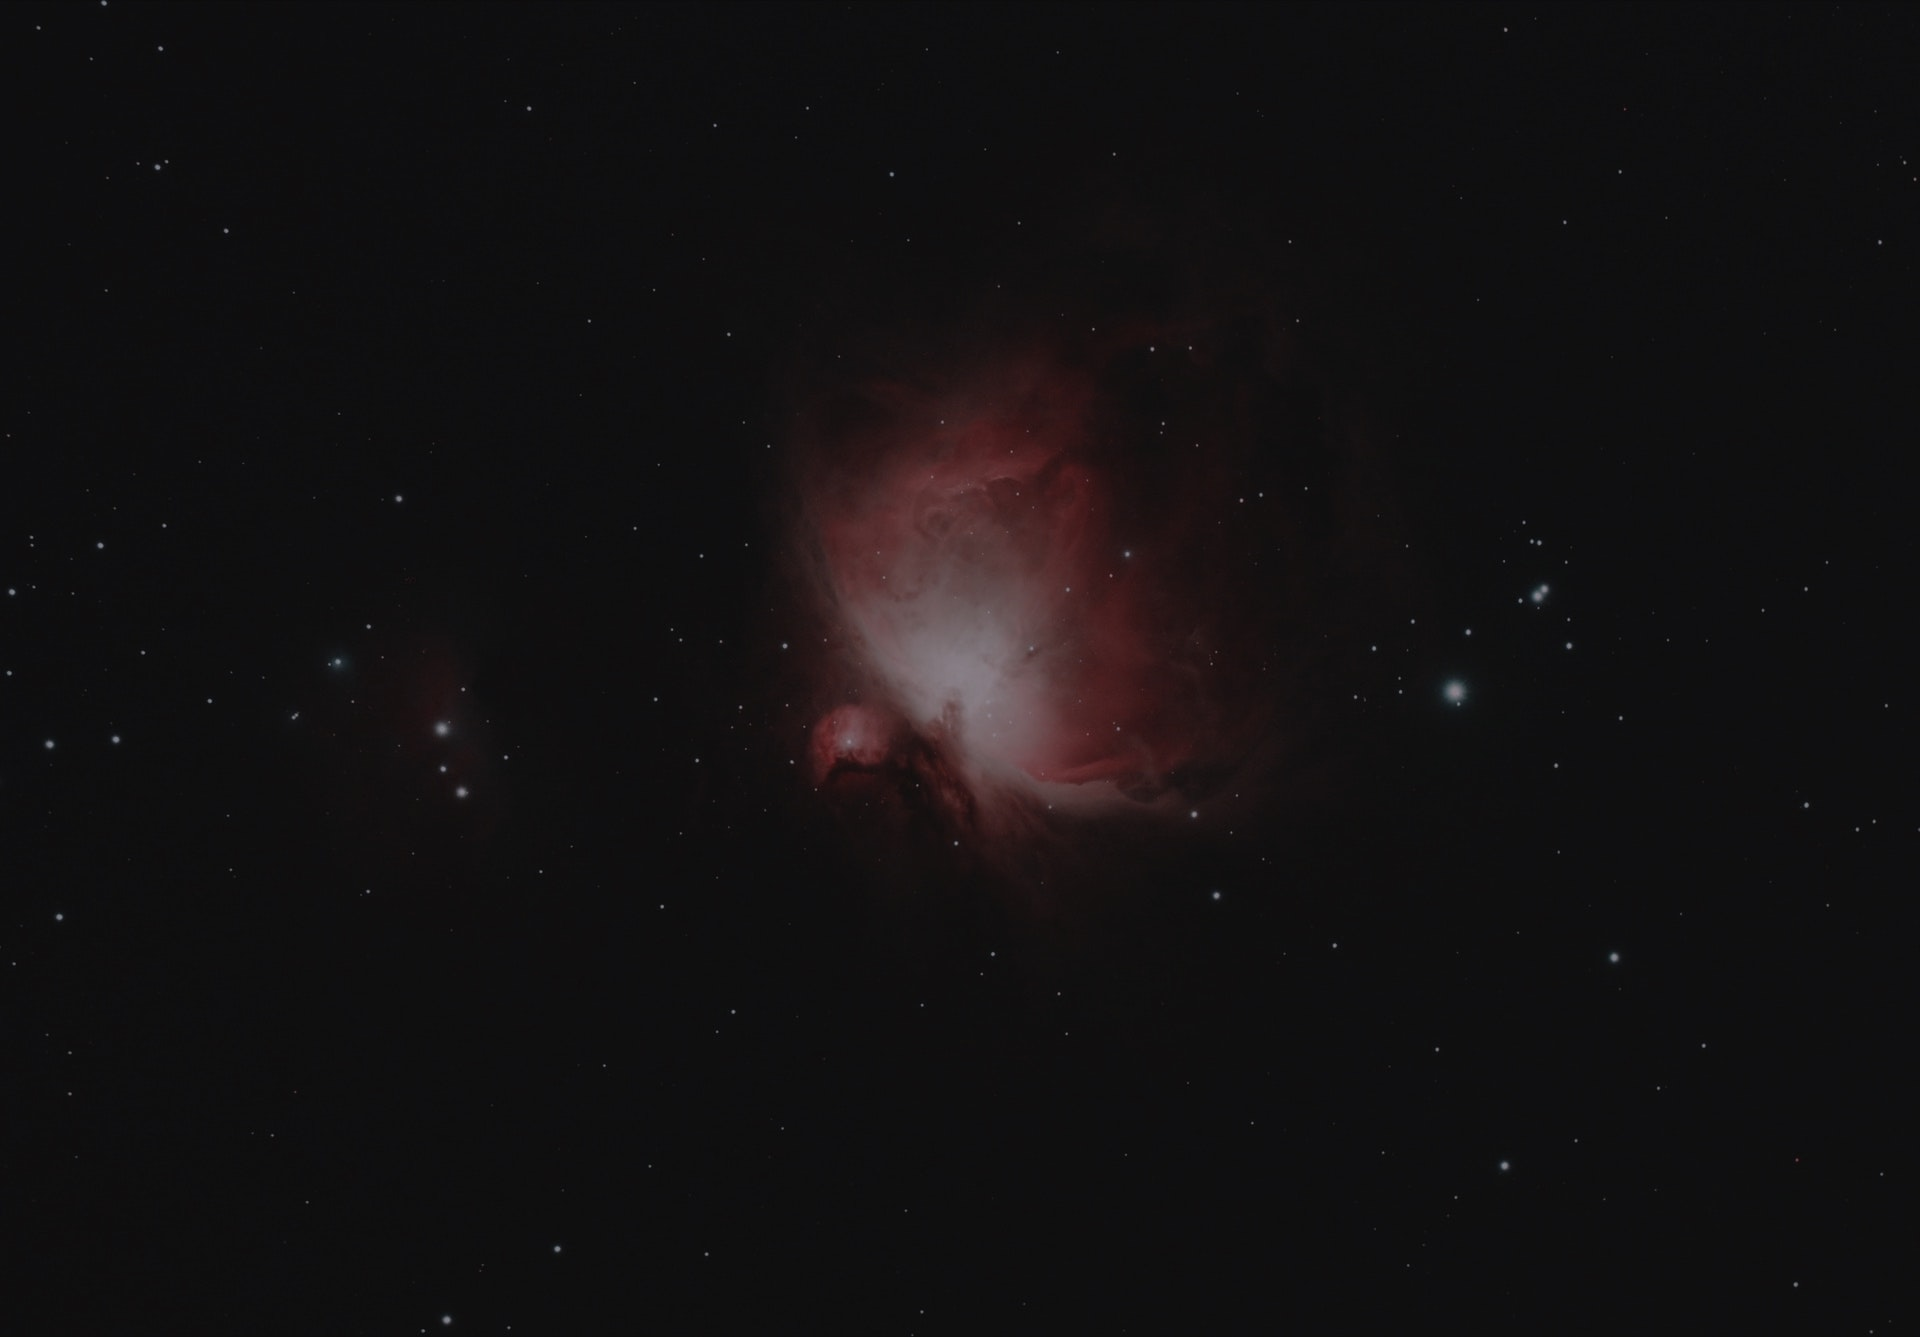
\includegraphics[width=\paperwidth]{./img/orion-nebula-copy.jpg}}

\begin{frame}%{Reconnaissance}
    \textbf{reconnaissance}: \textit{n}. 1. Military observation of a region to locate an enemy or ascertain strategic features. 2. Preliminary surveying or research.
\end{frame}

\begin{frame}
    \frametitle{General Approach}
    To test a web application for security vulnerabilities, you must first get to know it. You must understand what functions are used and what parameters are used by these functions. You have to test every parameter whether it can be exploited (e.g., using illegitimate values). You also need to check whether the web application code contains known vulnerabilities.
    

\end{frame}

\begin{frame}
    \frametitle{Sample frame title}
    
    In this slide, some important text will be
    \alert{highlighted} because it's important.
    Please, don't abuse it.
    
    \begin{block}{Remark}
    Sample text
    \end{block}
    
    \begin{alertblock}{Important theorem}
    Sample text in red box
    \end{alertblock}
    
    \begin{examples}
    Sample text in green box. The title of the block is ``Examples".
    \end{examples}

\end{frame}

\begin{frame}
    \frametitle{Tools}
    \begin{itemize}
        \item ZAProxy
        \item ...
    \end{itemize}
\end{frame}


\begin{frame}
    \frametitle{Example}

    \begin{itemize}
        \item<1-> one
        \item<2-> two
        \item<3-> theorem
    \end{itemize}

\end{frame}

\begin{frame}
    \frametitle{Example 1}
    One \pause
    Two \pause
    Three
\end{frame}

\section{0x3: Stateful Attacks}
{
\usebackgroundtemplate{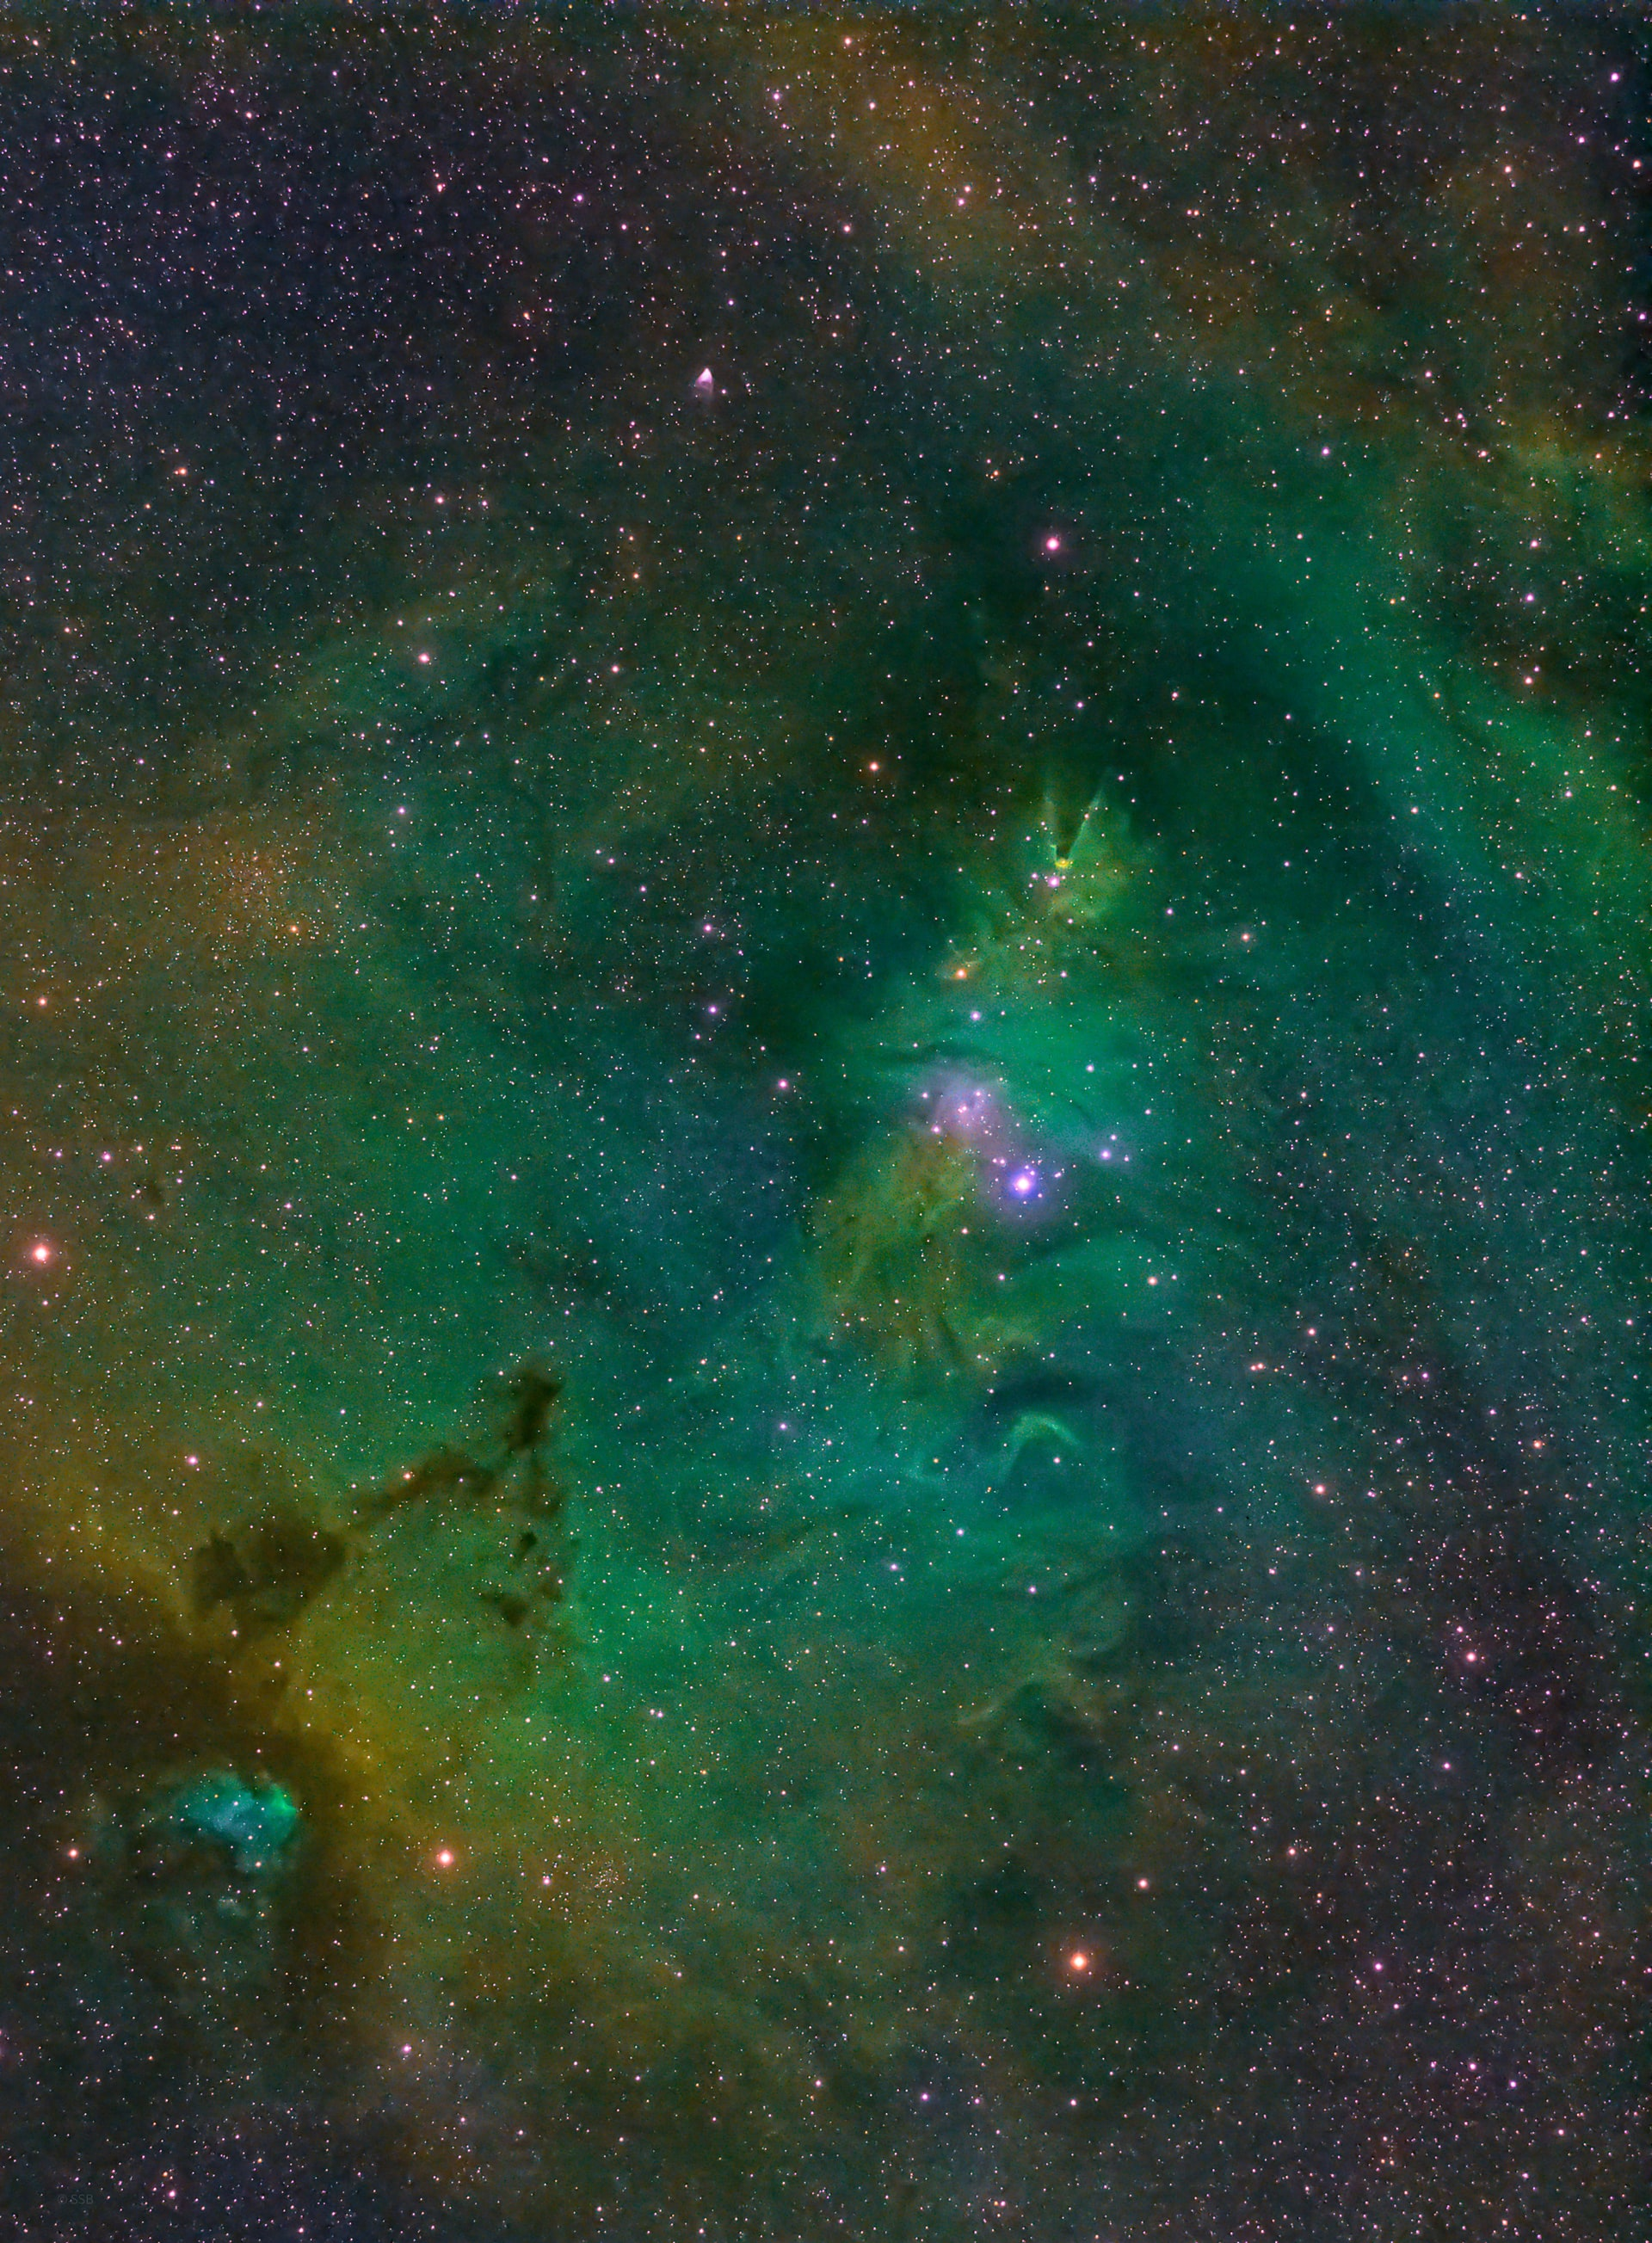
\includegraphics[width=\paperwidth]{./img/aldebaran.jpg}}
\begin{frame}
\huge{\textcolor{white}{\textbf{0x3: Stateful Attacks}}}
\end{frame}
}

\section{0x4: Attacks on Authentication}
{
\usebackgroundtemplate{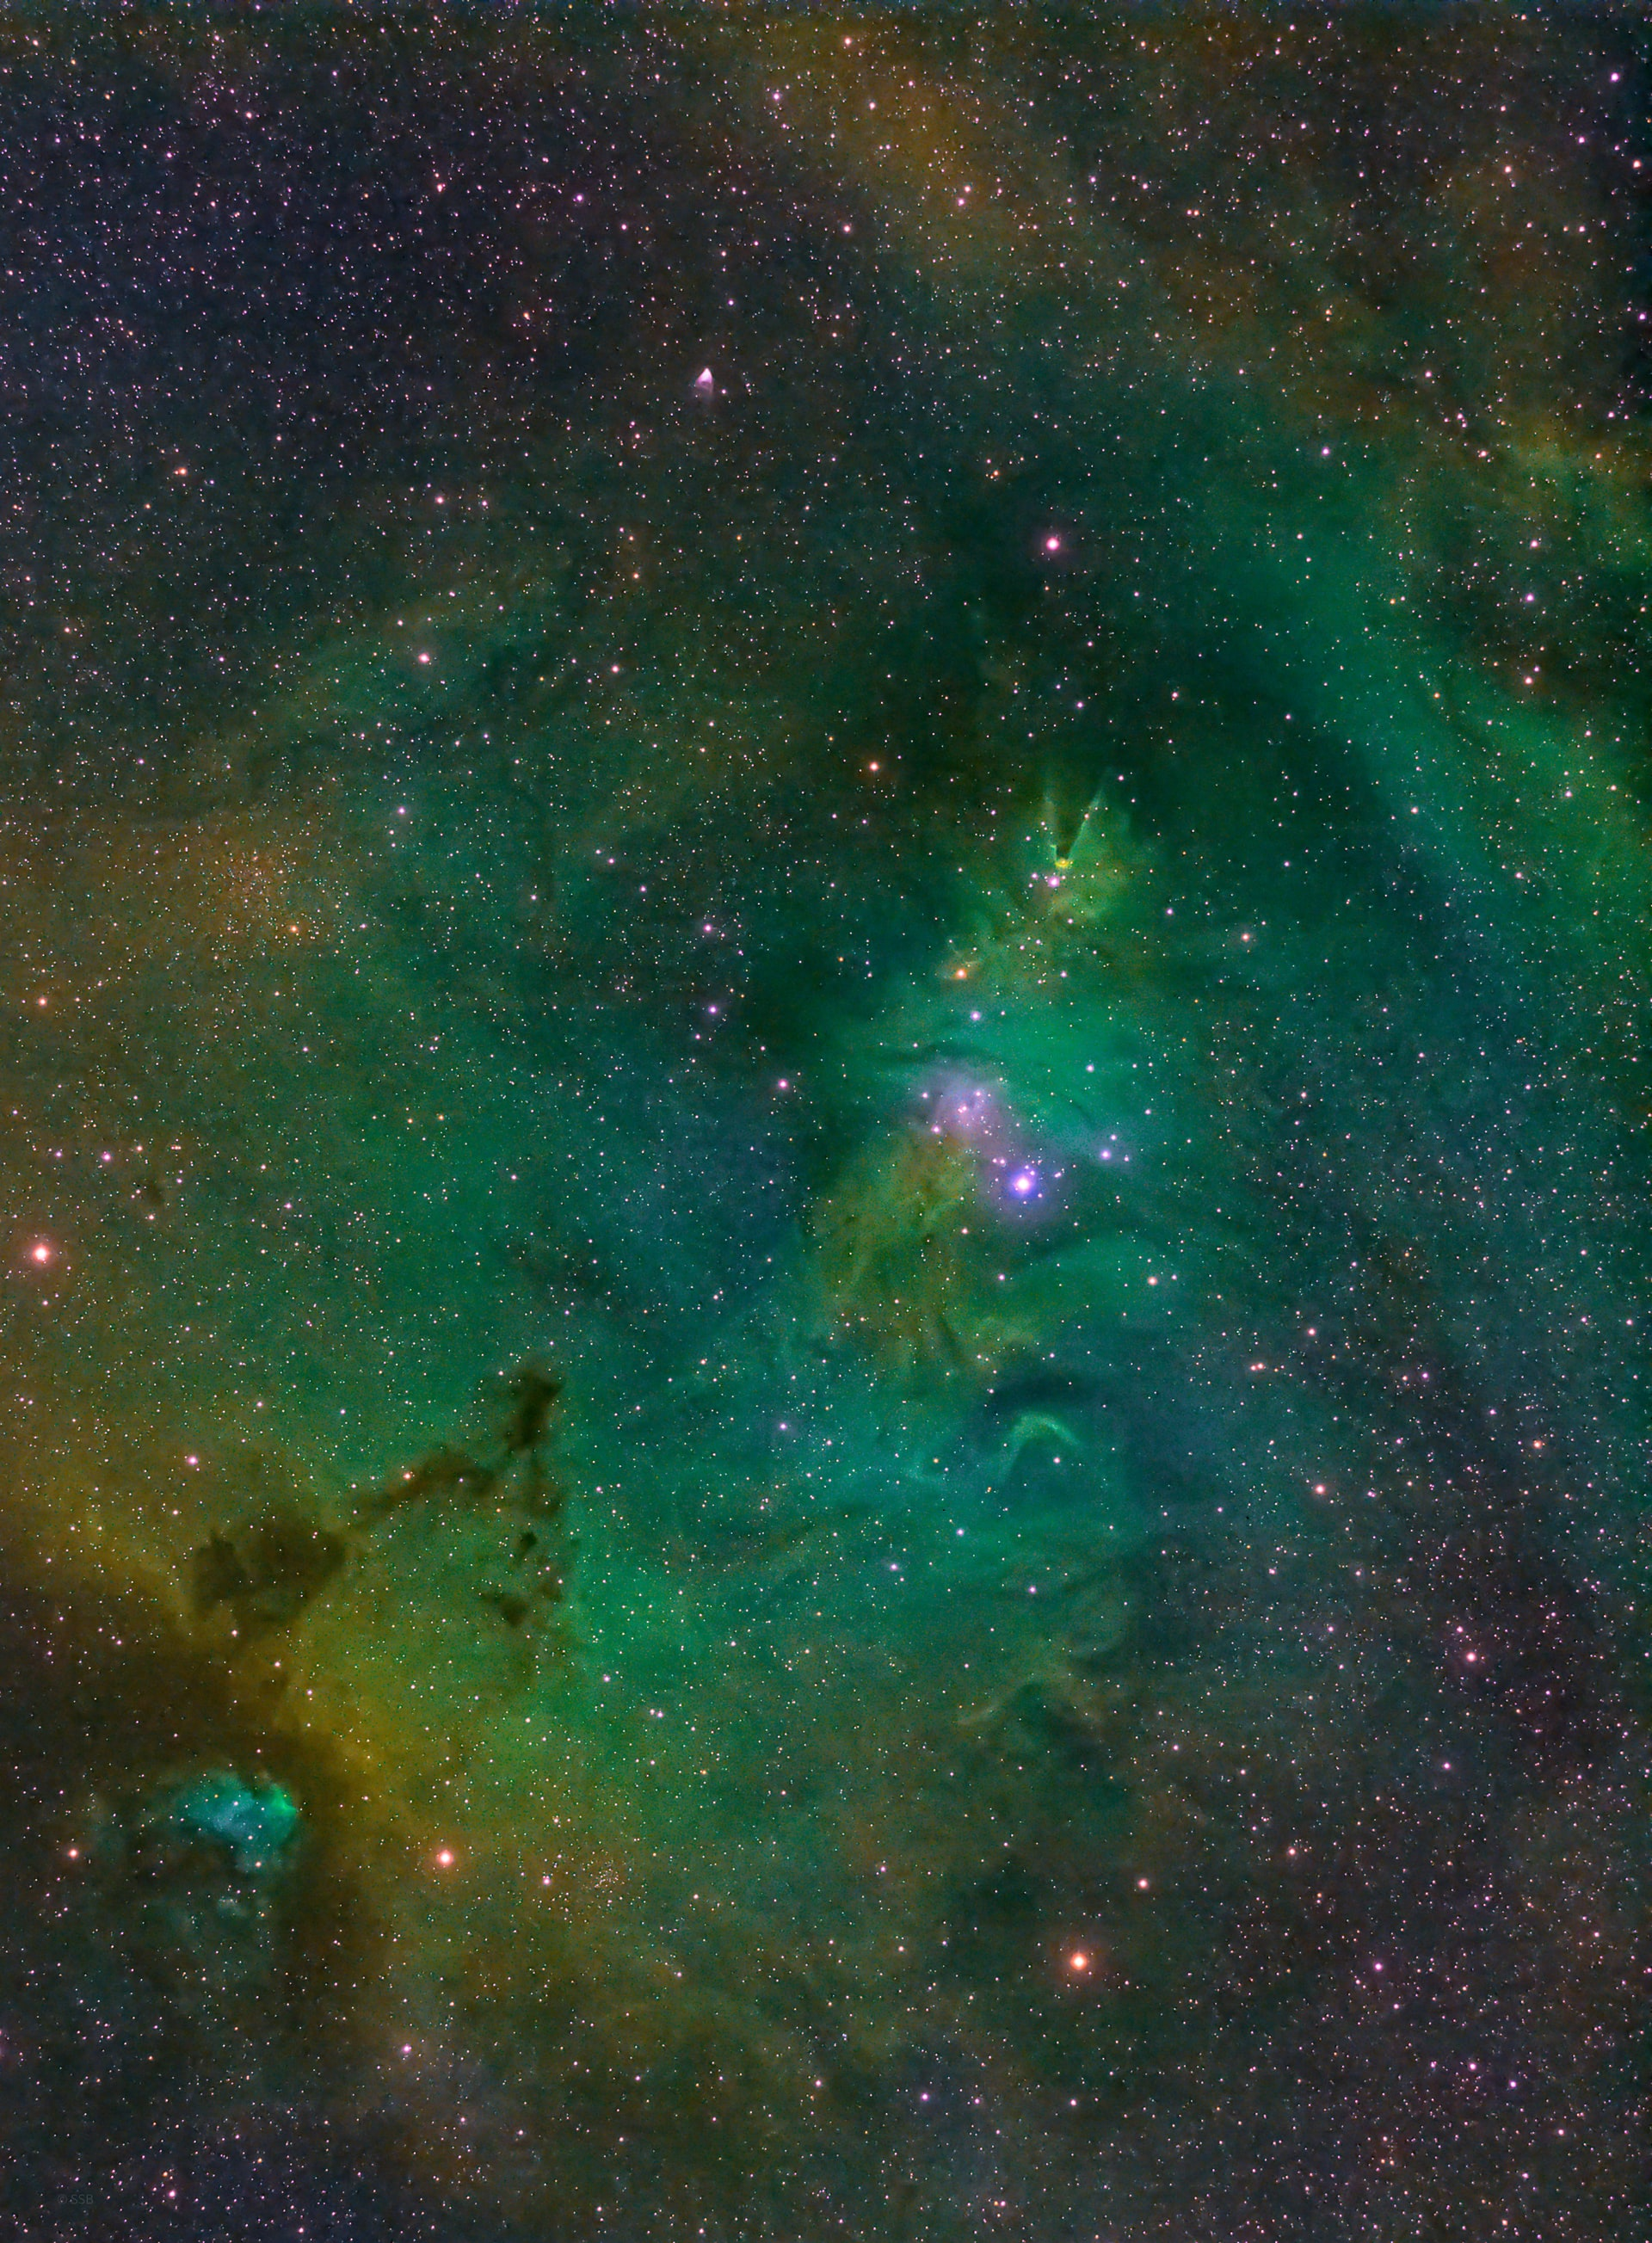
\includegraphics[width=\paperwidth]{./img/aldebaran.jpg}}
\begin{frame}
\huge{\textcolor{white}{\textbf{0x4: Attacks on Authentication}}}
\end{frame}
}

\section{0x5: Cross-Site-Scripting (XSS)}
{
\usebackgroundtemplate{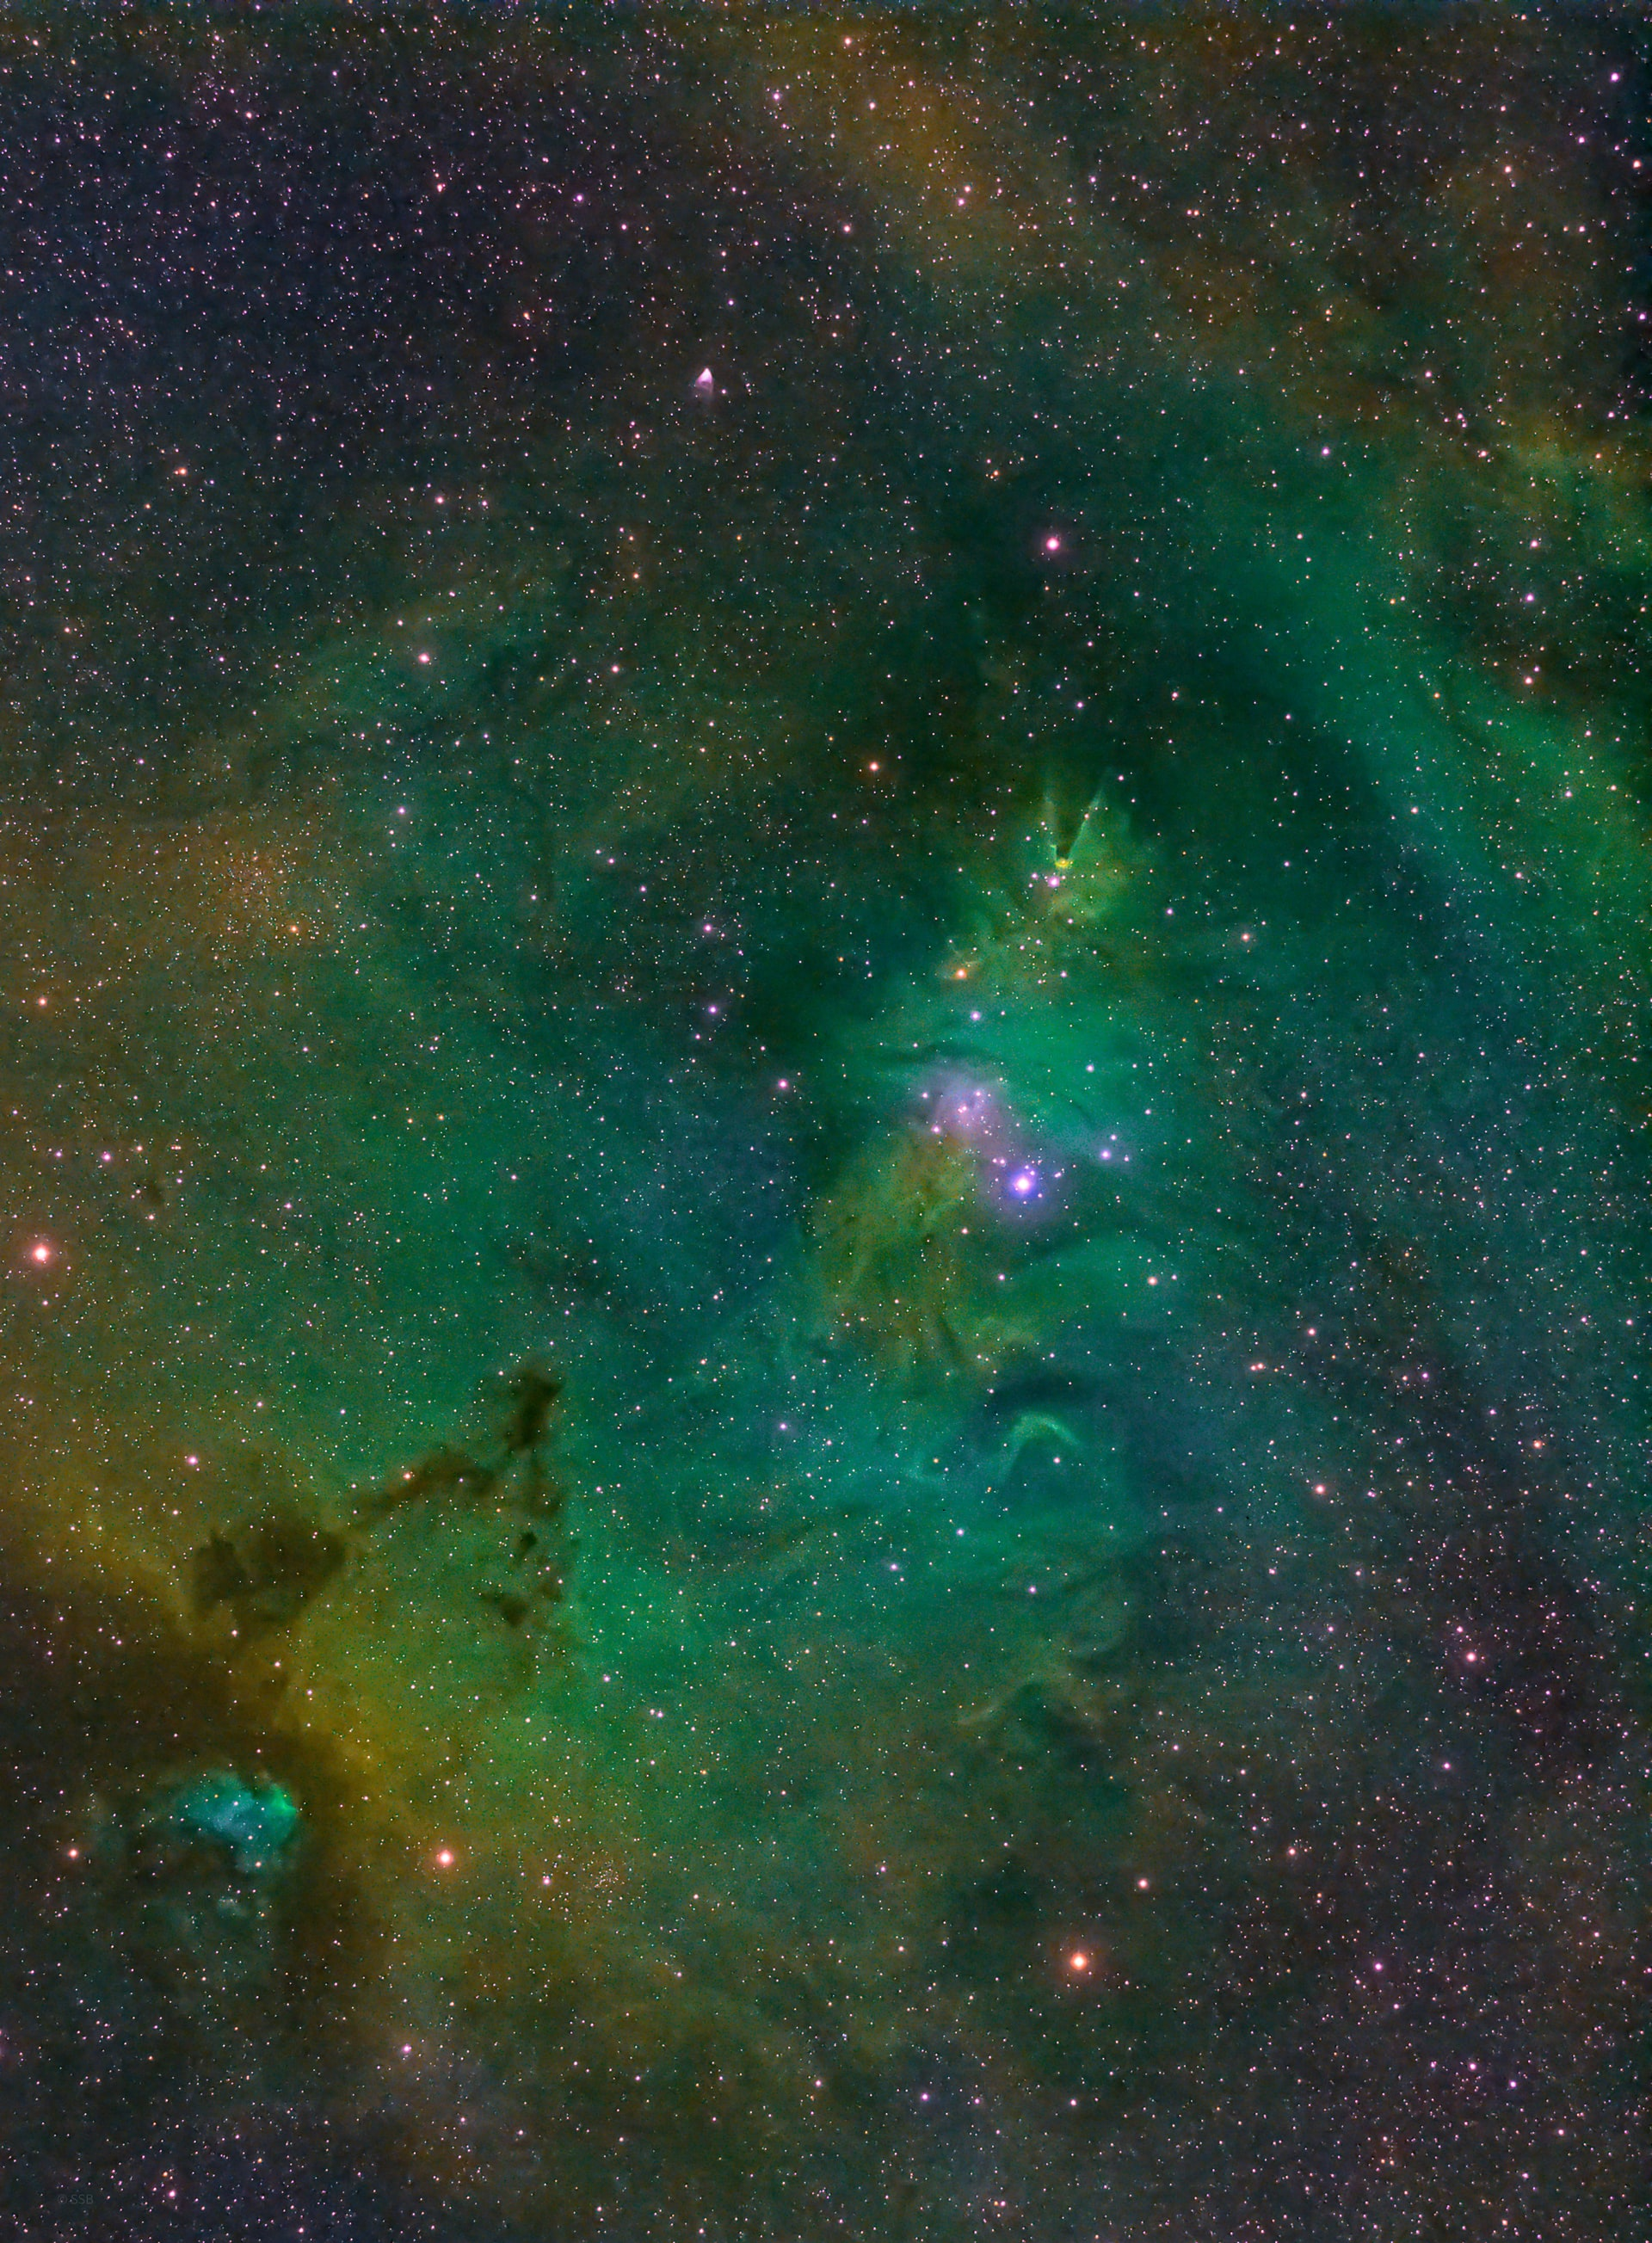
\includegraphics[width=\paperwidth]{./img/aldebaran.jpg}}
\begin{frame}
\huge{\textcolor{white}{\textbf{0x5: Cross-Site-Scripting (XSS)}}}
\end{frame}
}

\section{0x6: SQL Injection}
{
\usebackgroundtemplate{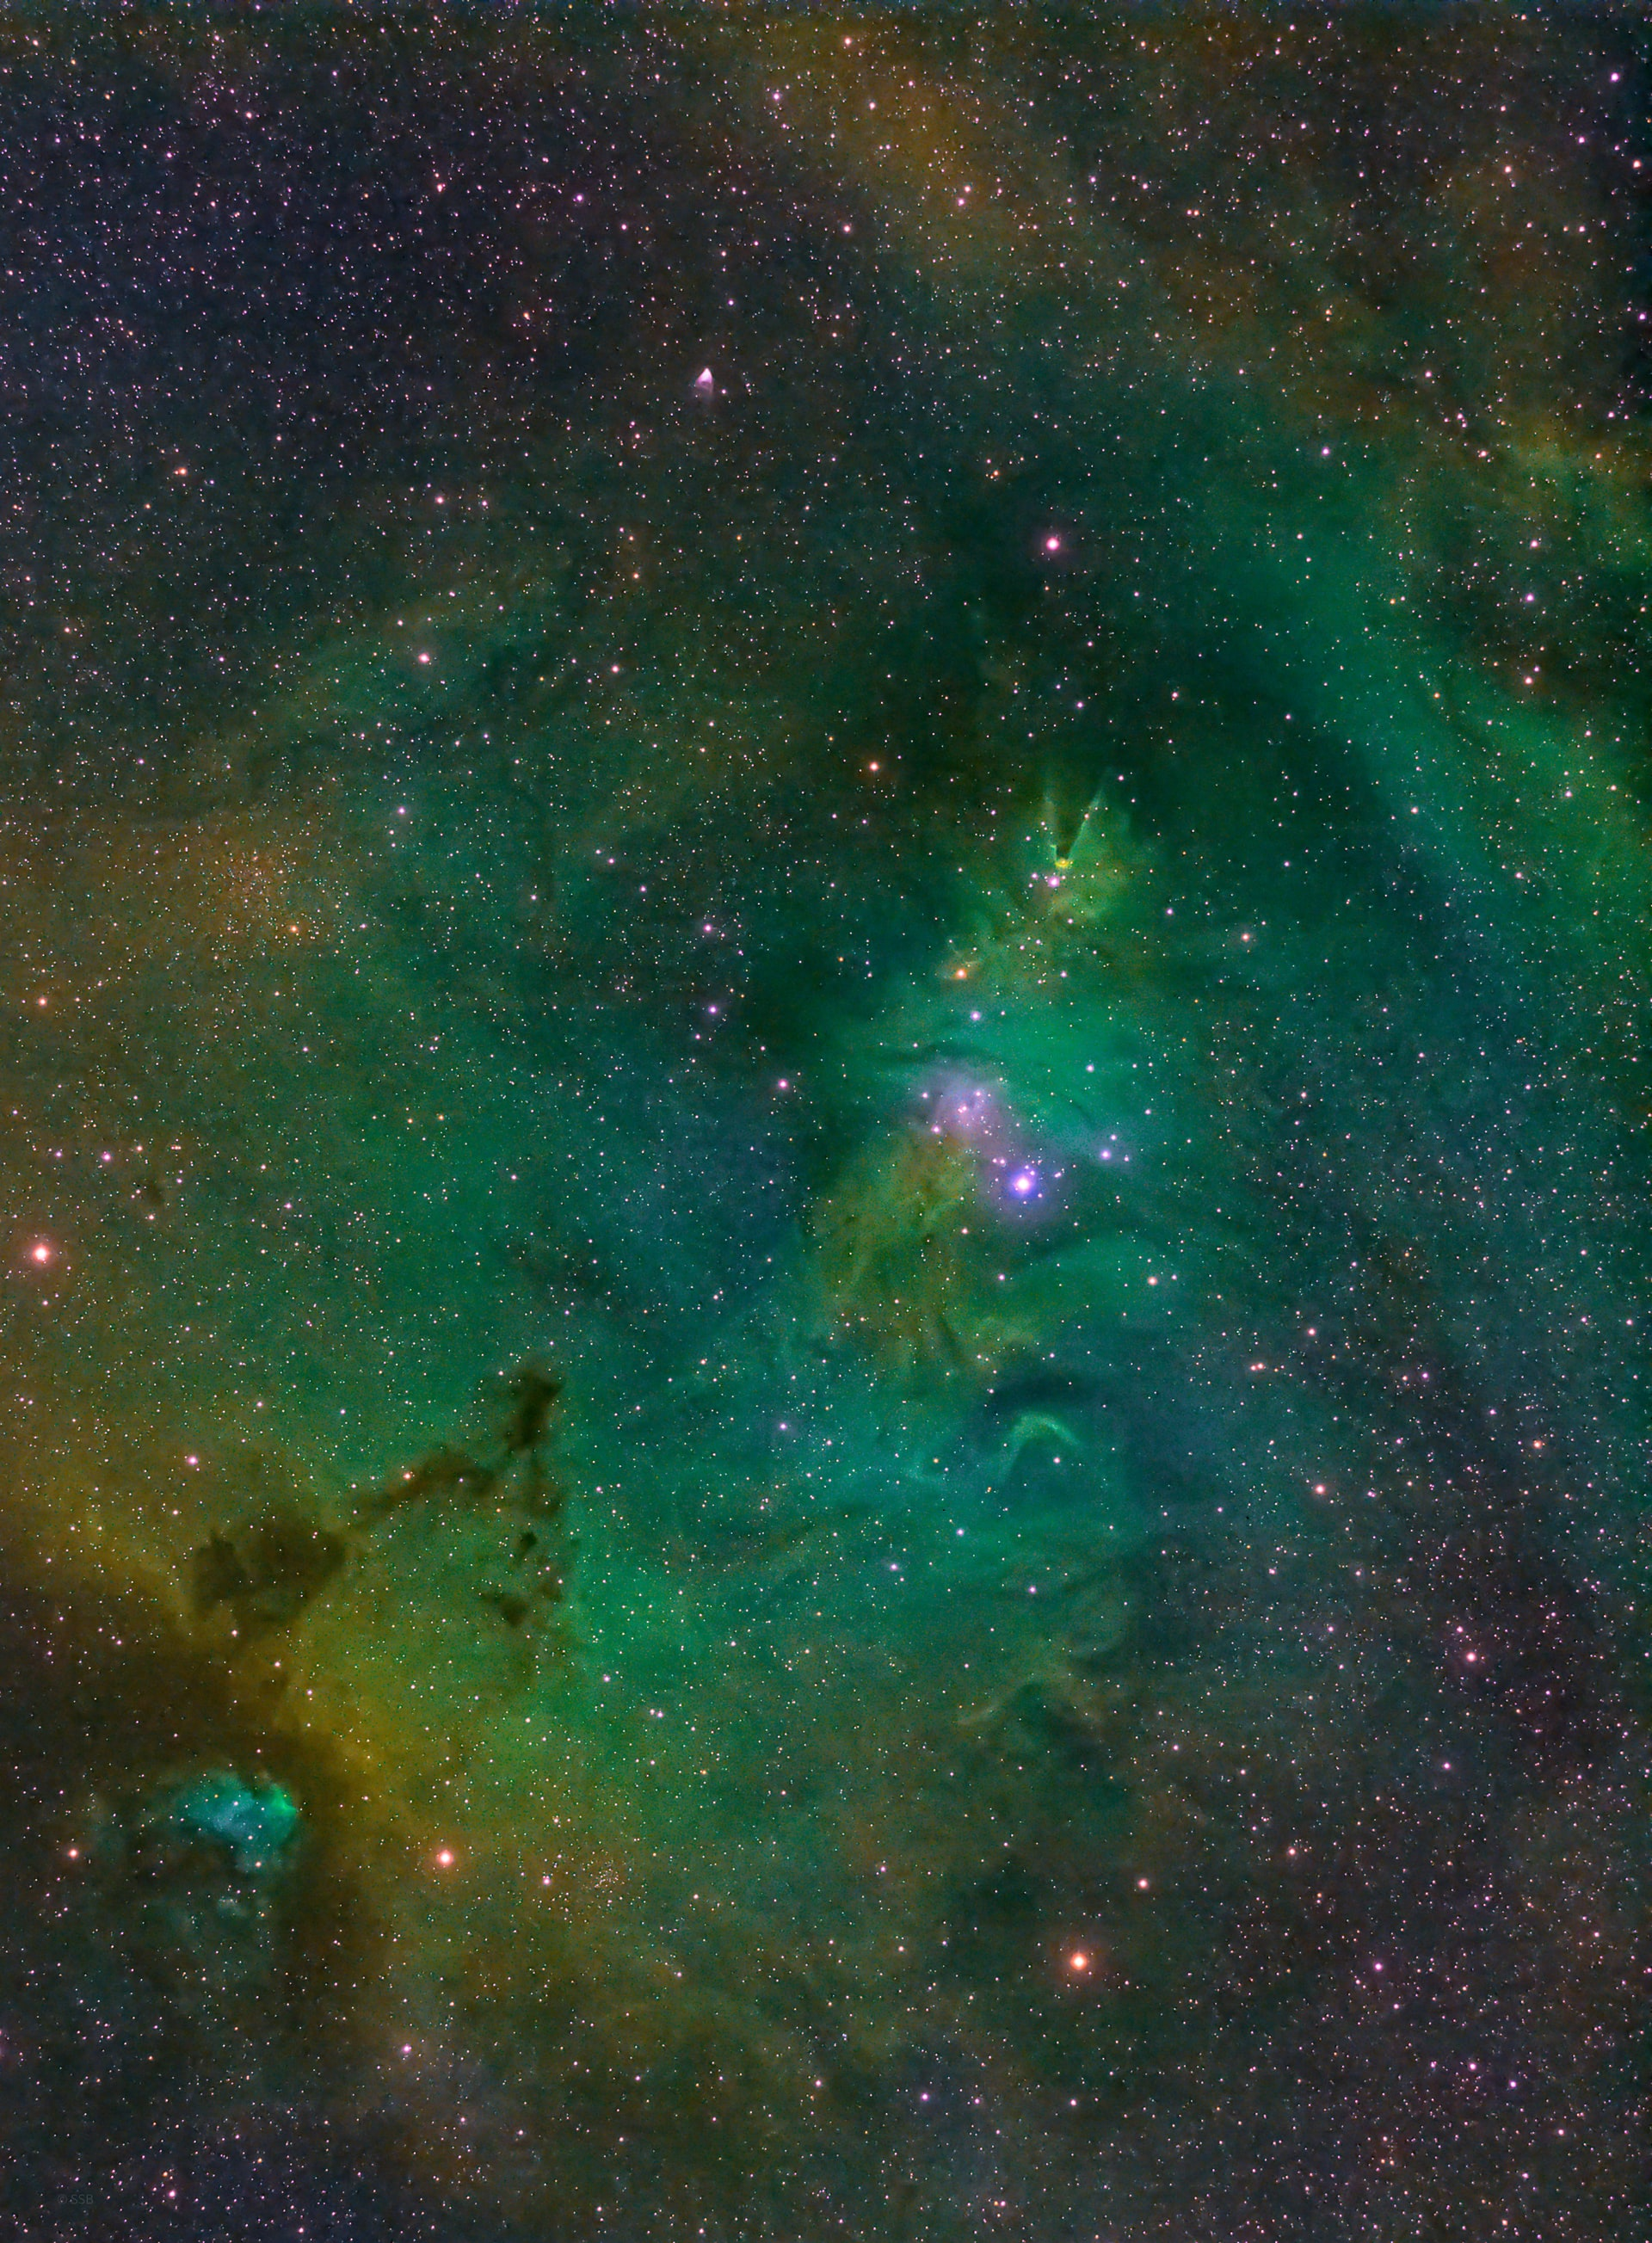
\includegraphics[width=\paperwidth]{./img/aldebaran.jpg}}
\begin{frame}
\huge{\textcolor{white}{\textbf{0x6: SQL Injection}}}
\end{frame}
}

\section{0x7: Other Injection-Based Vulnerabilities}
{
\usebackgroundtemplate{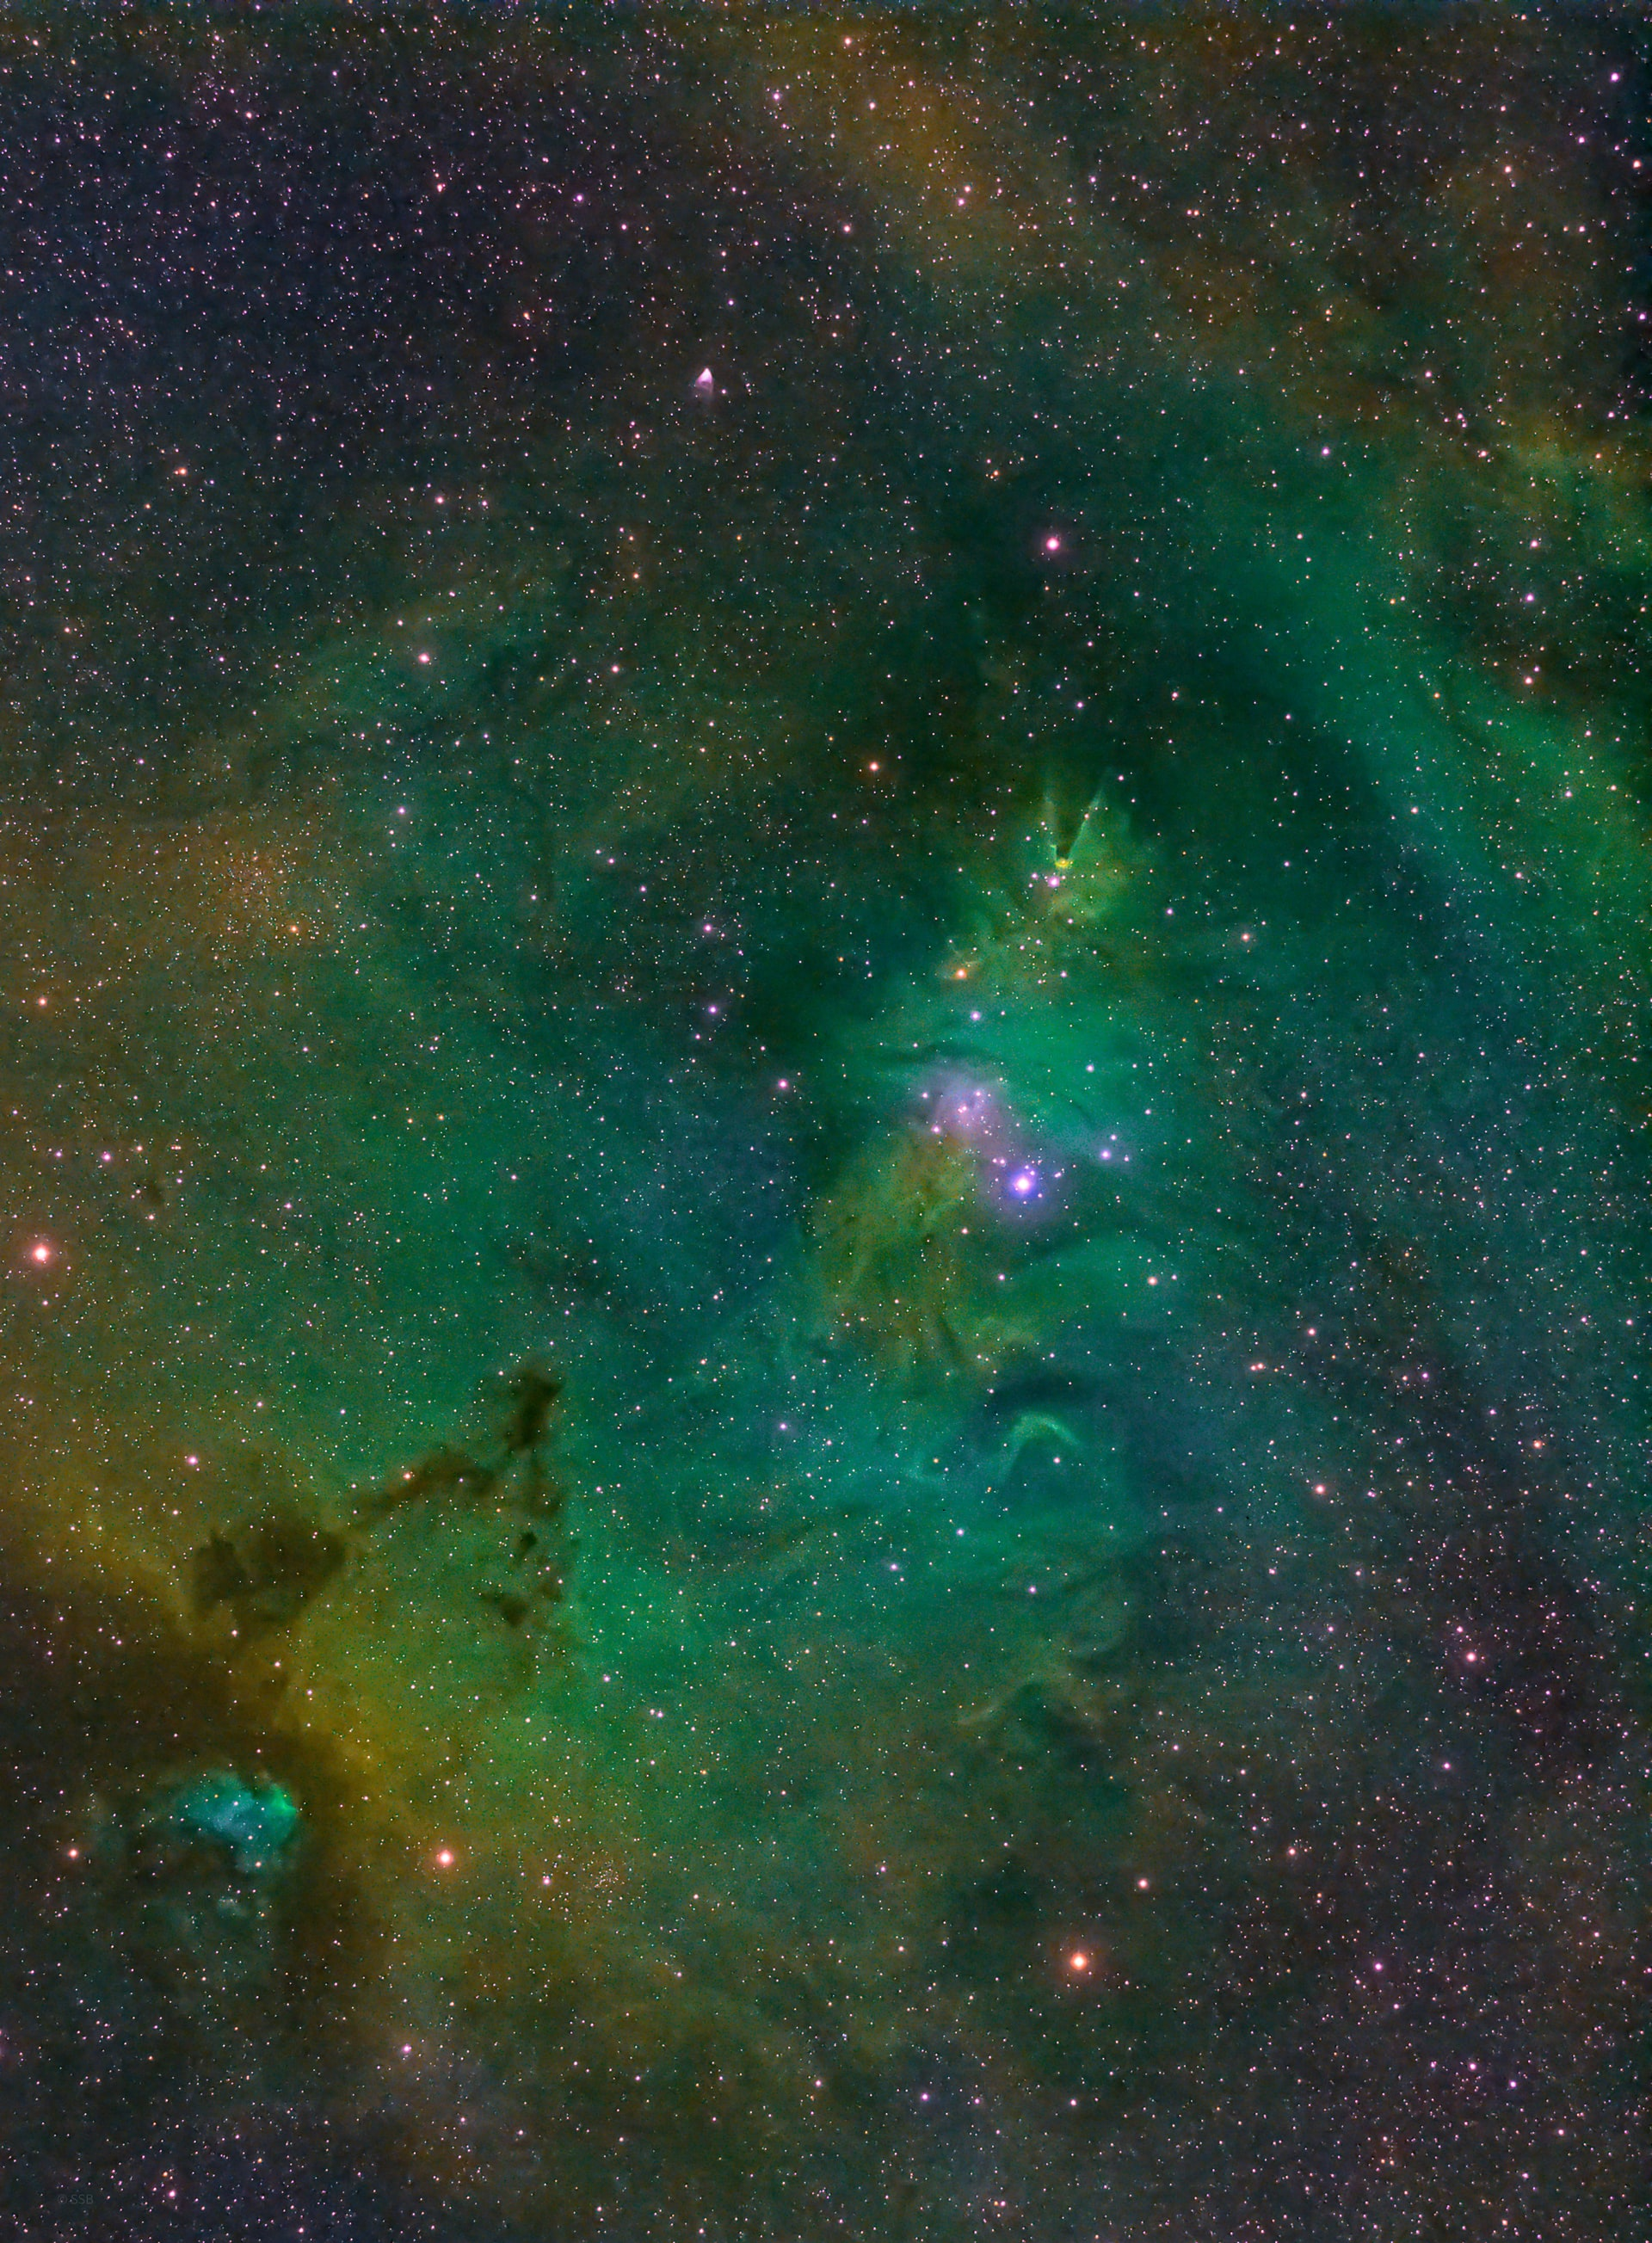
\includegraphics[width=\paperwidth]{./img/aldebaran.jpg}}
\begin{frame}
\huge{\textcolor{white}{\textbf{0x7: Other Injection-Based Vulnerabilities}}}
\end{frame}
}

\section{0x8: Attacks on File Operations}
{
\usebackgroundtemplate{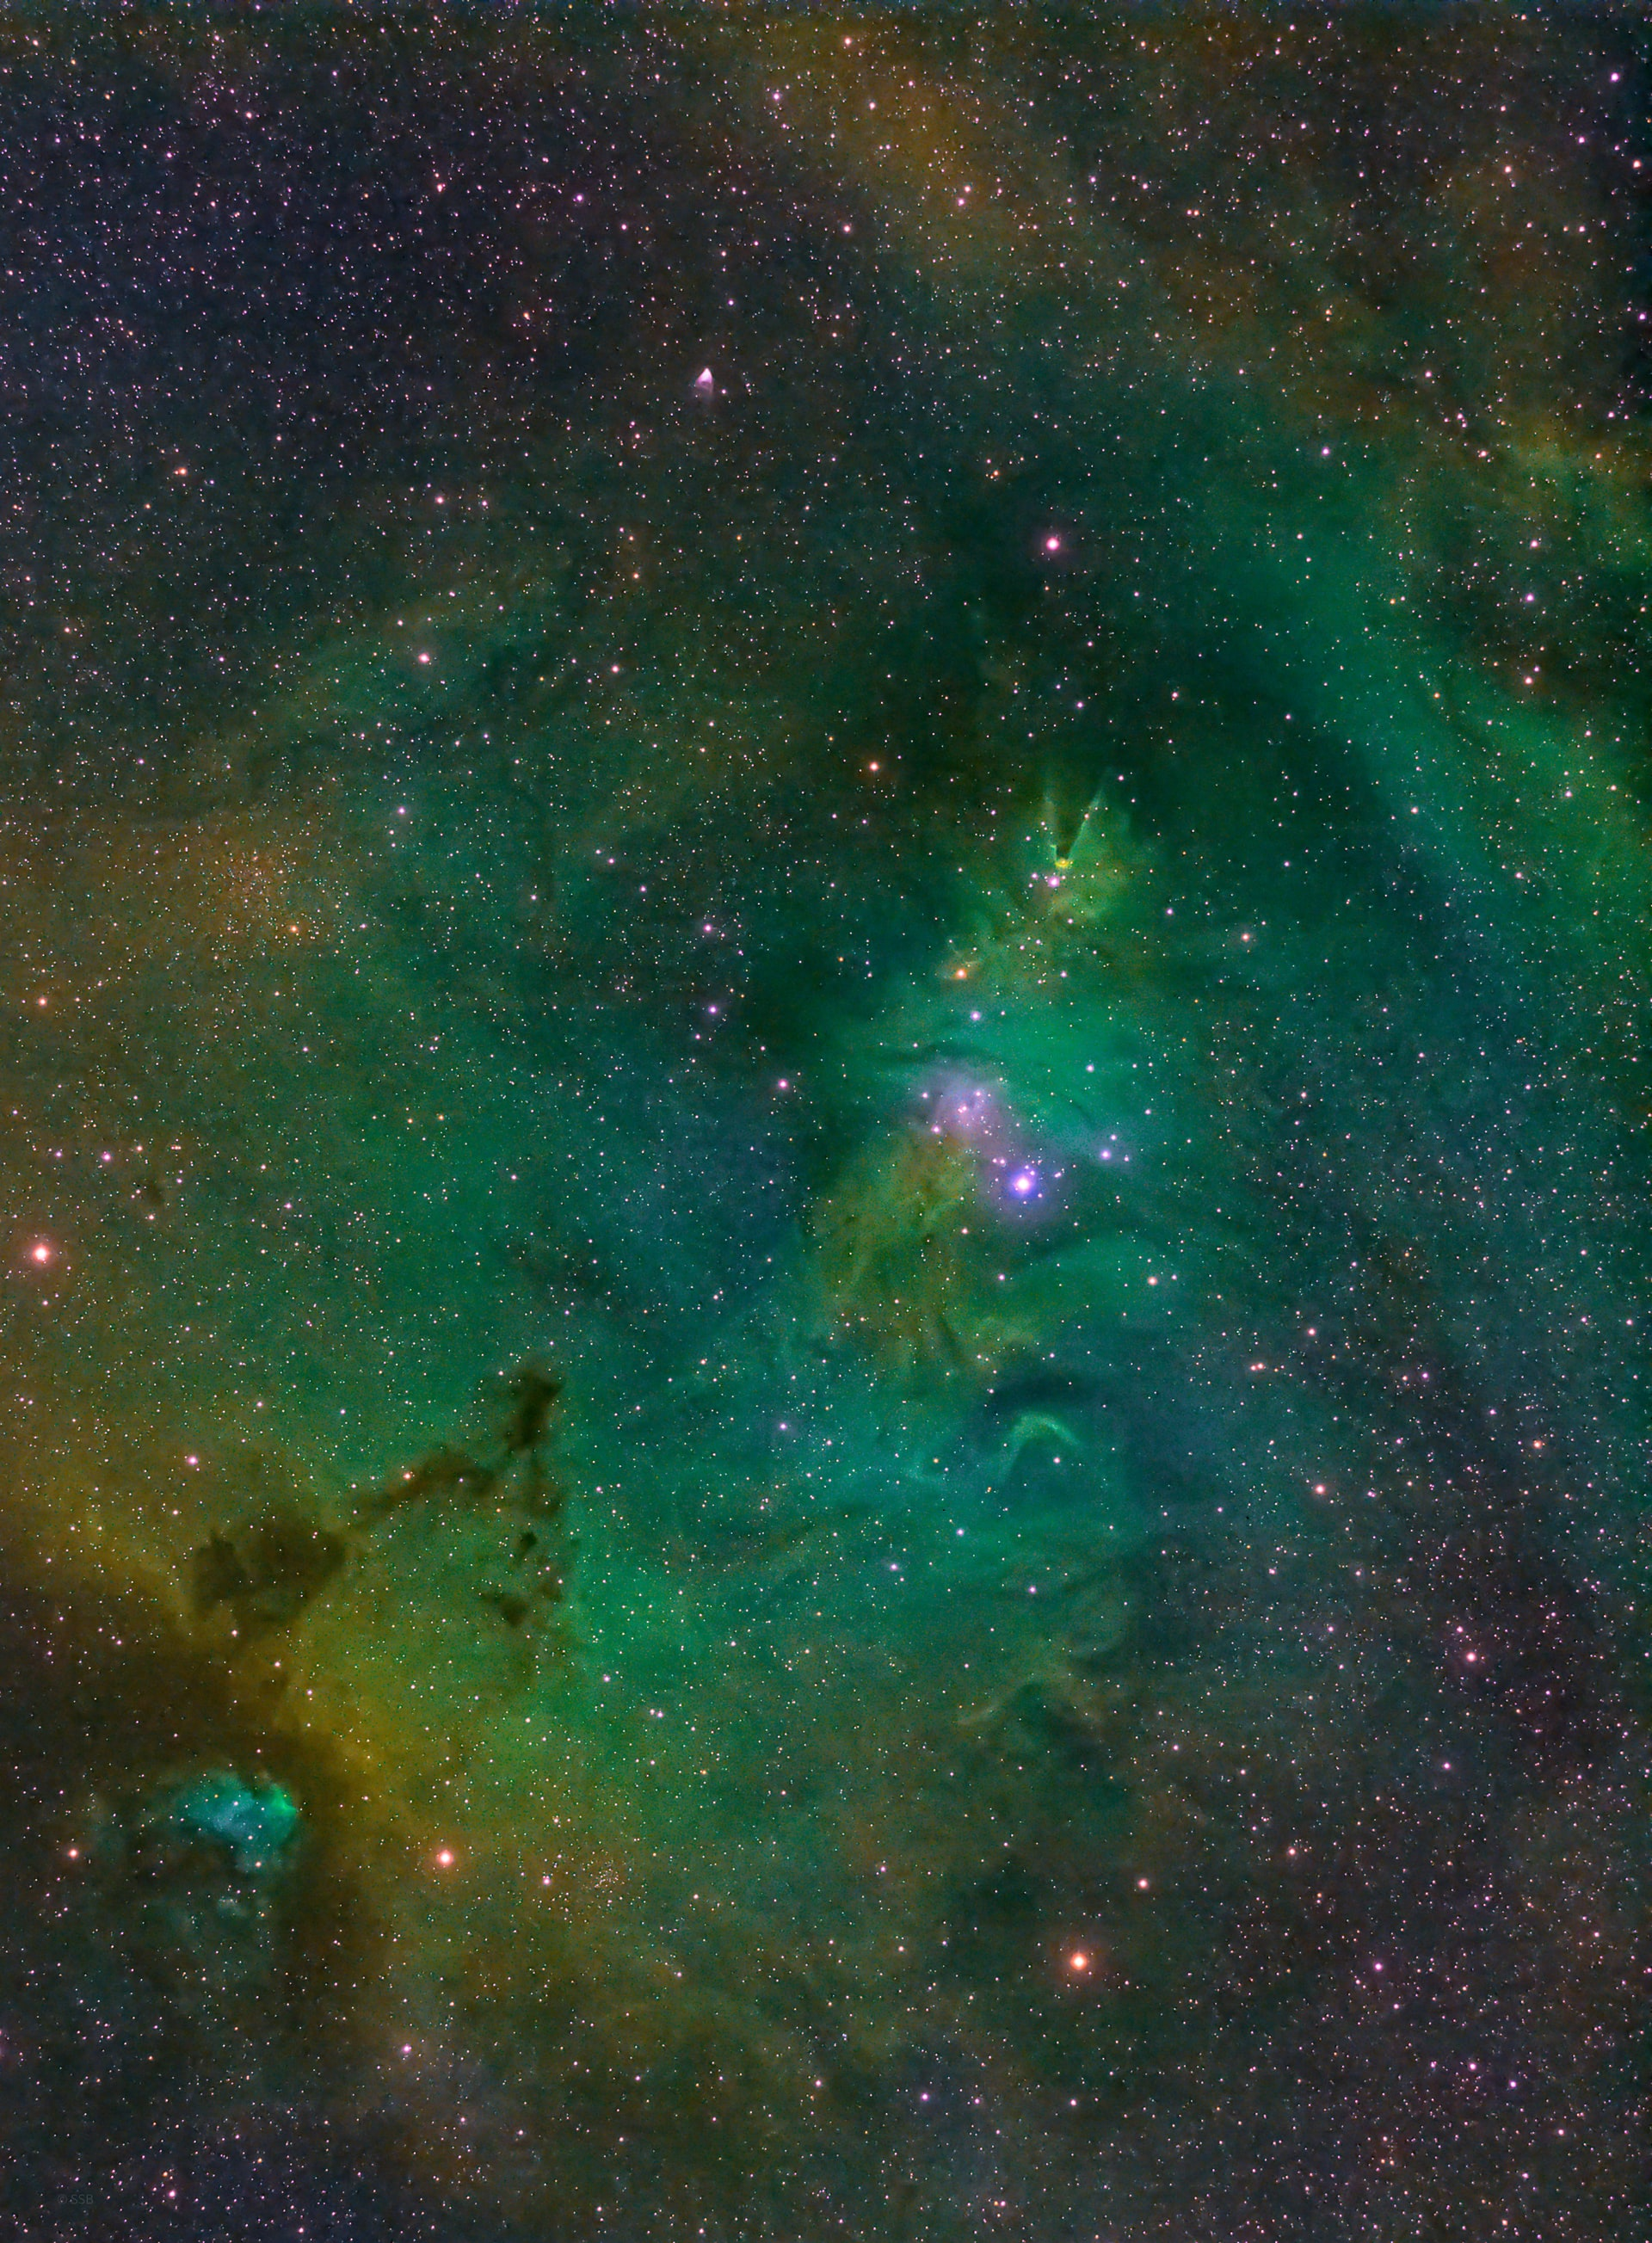
\includegraphics[width=\paperwidth]{./img/aldebaran.jpg}}
\begin{frame}
\huge{\textcolor{white}{\textbf{0x8: Attacks on File Operations}}}
\end{frame}
}

\section{0x9: Buffer Overflows, Format Strings and Integer Bugs}
{
\usebackgroundtemplate{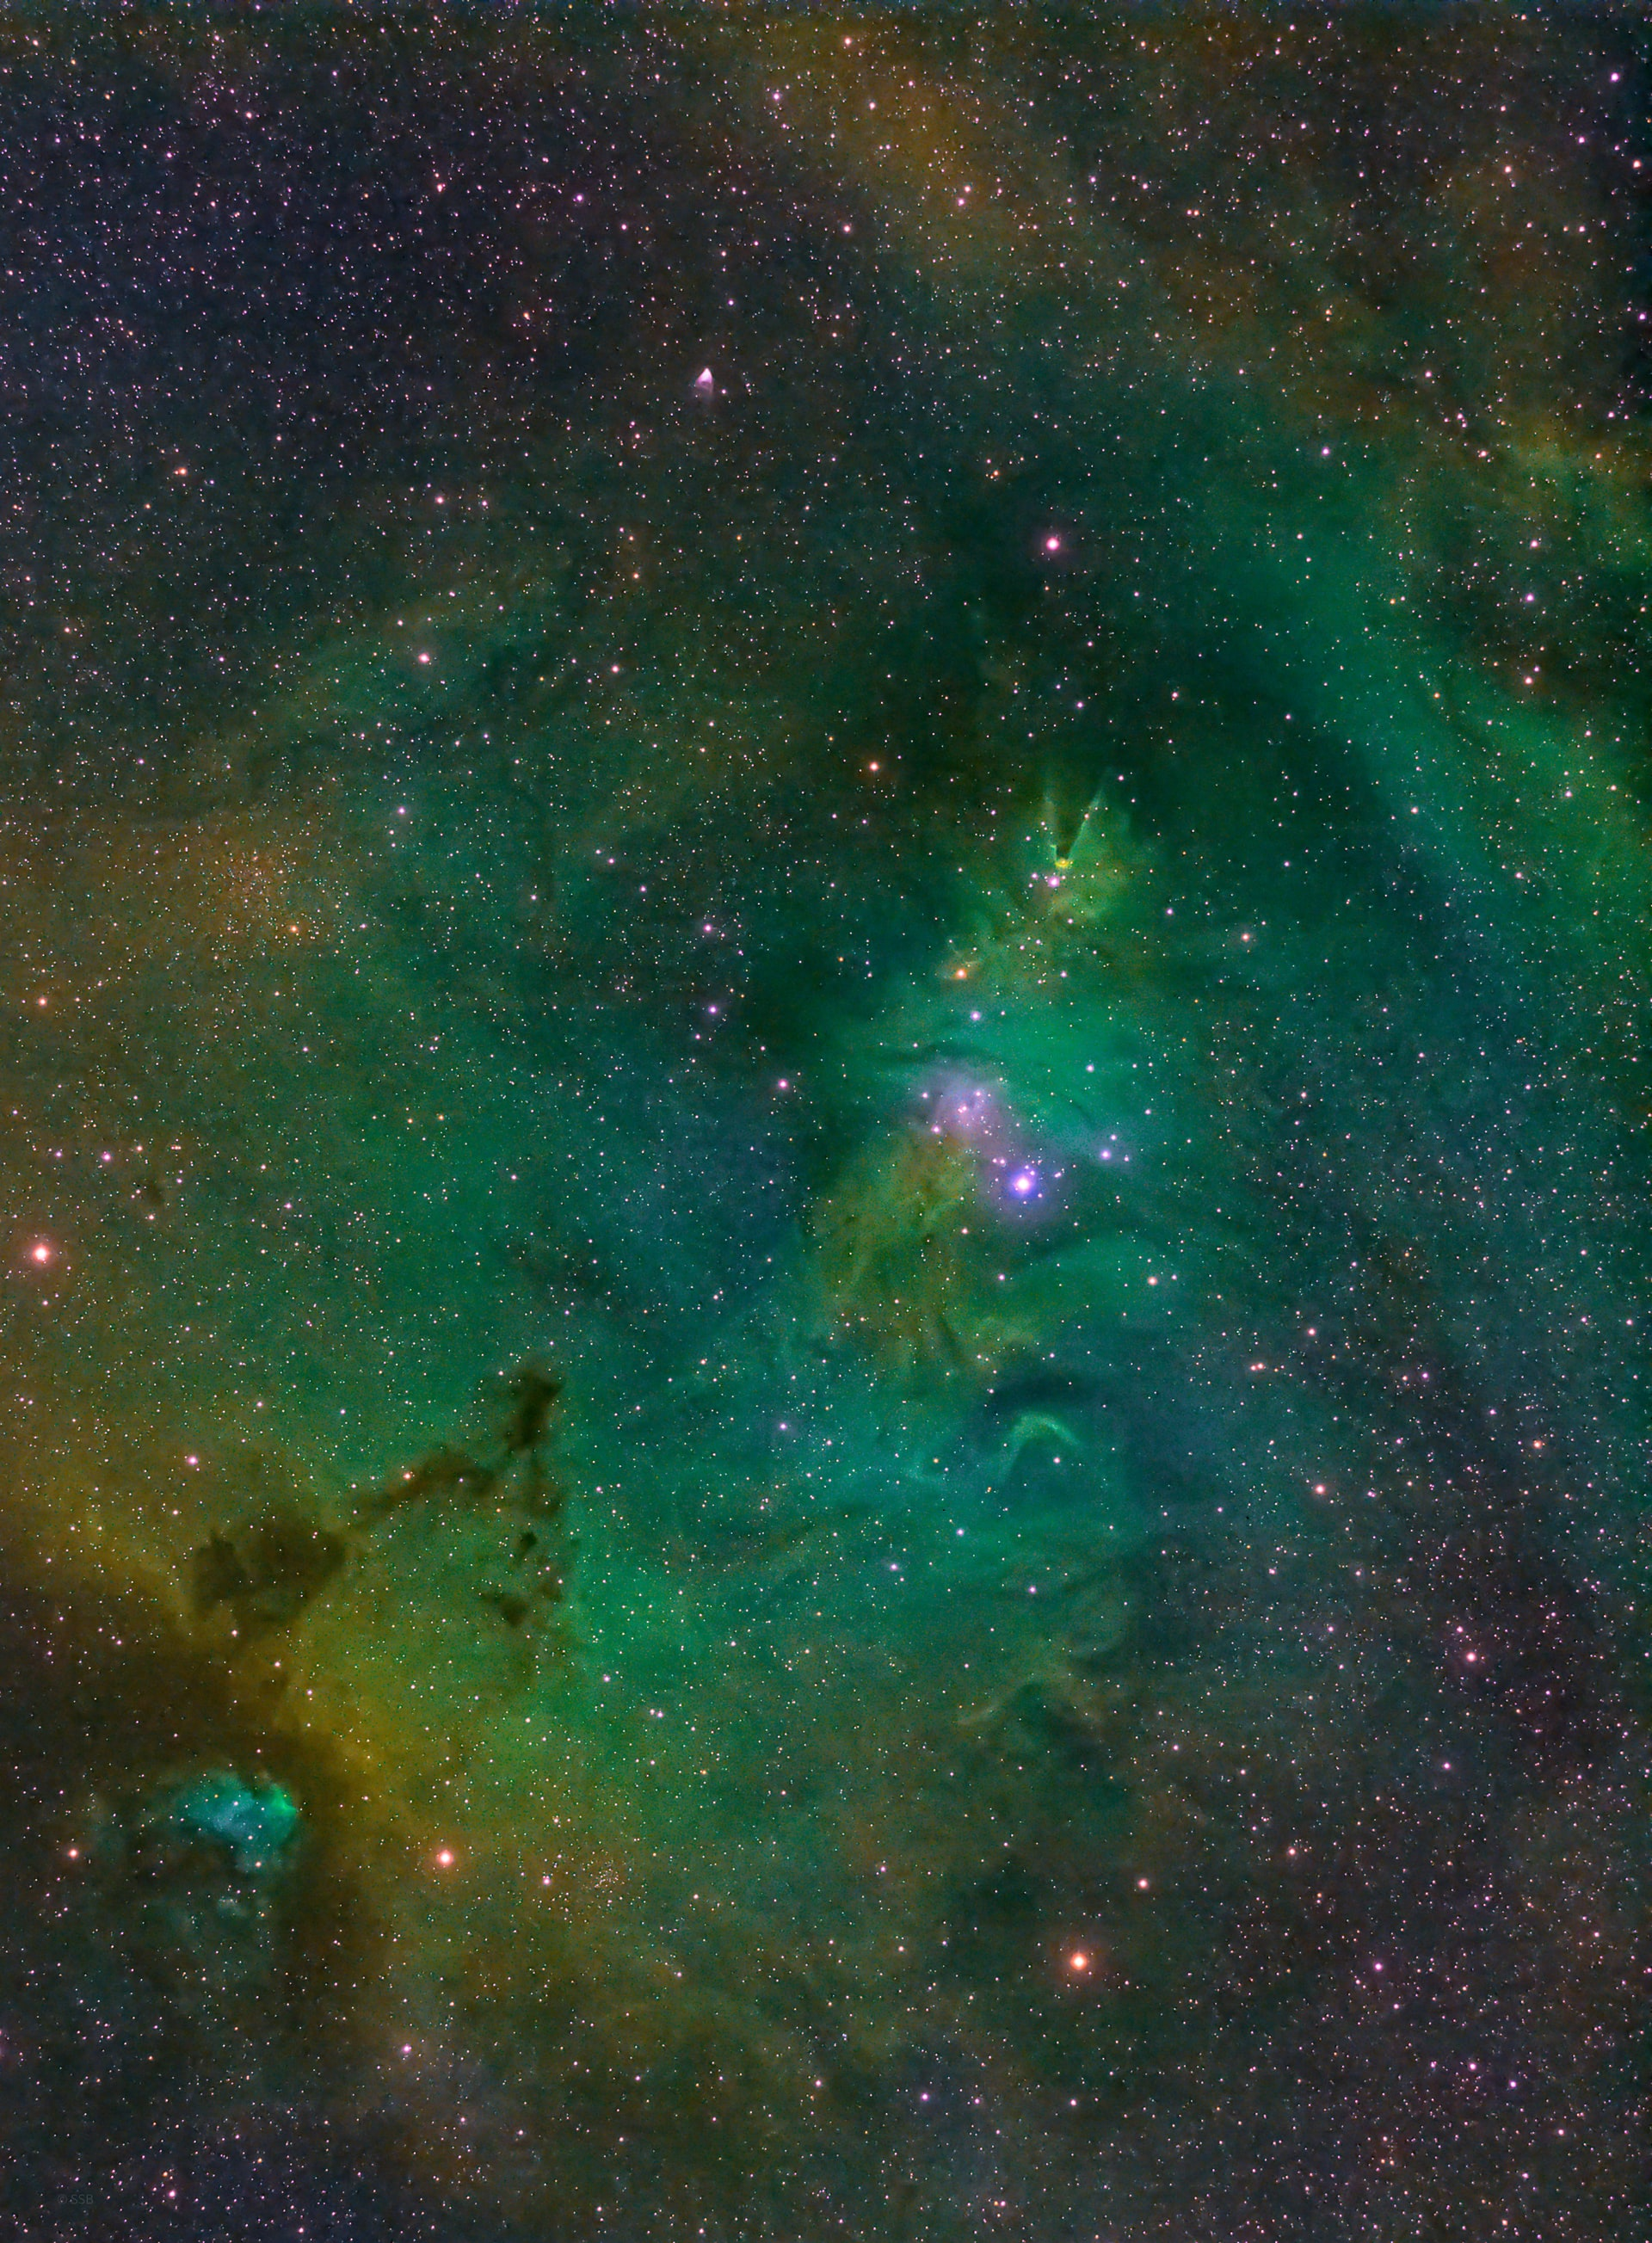
\includegraphics[width=\paperwidth]{./img/aldebaran.jpg}}
\begin{frame}
\huge{\textcolor{white}{\textbf{0x9: Buffer Overflows, Format Strings and Integer Bugs}}}
\end{frame}
}

\section{0xA: Architectural Attacks}
{
\usebackgroundtemplate{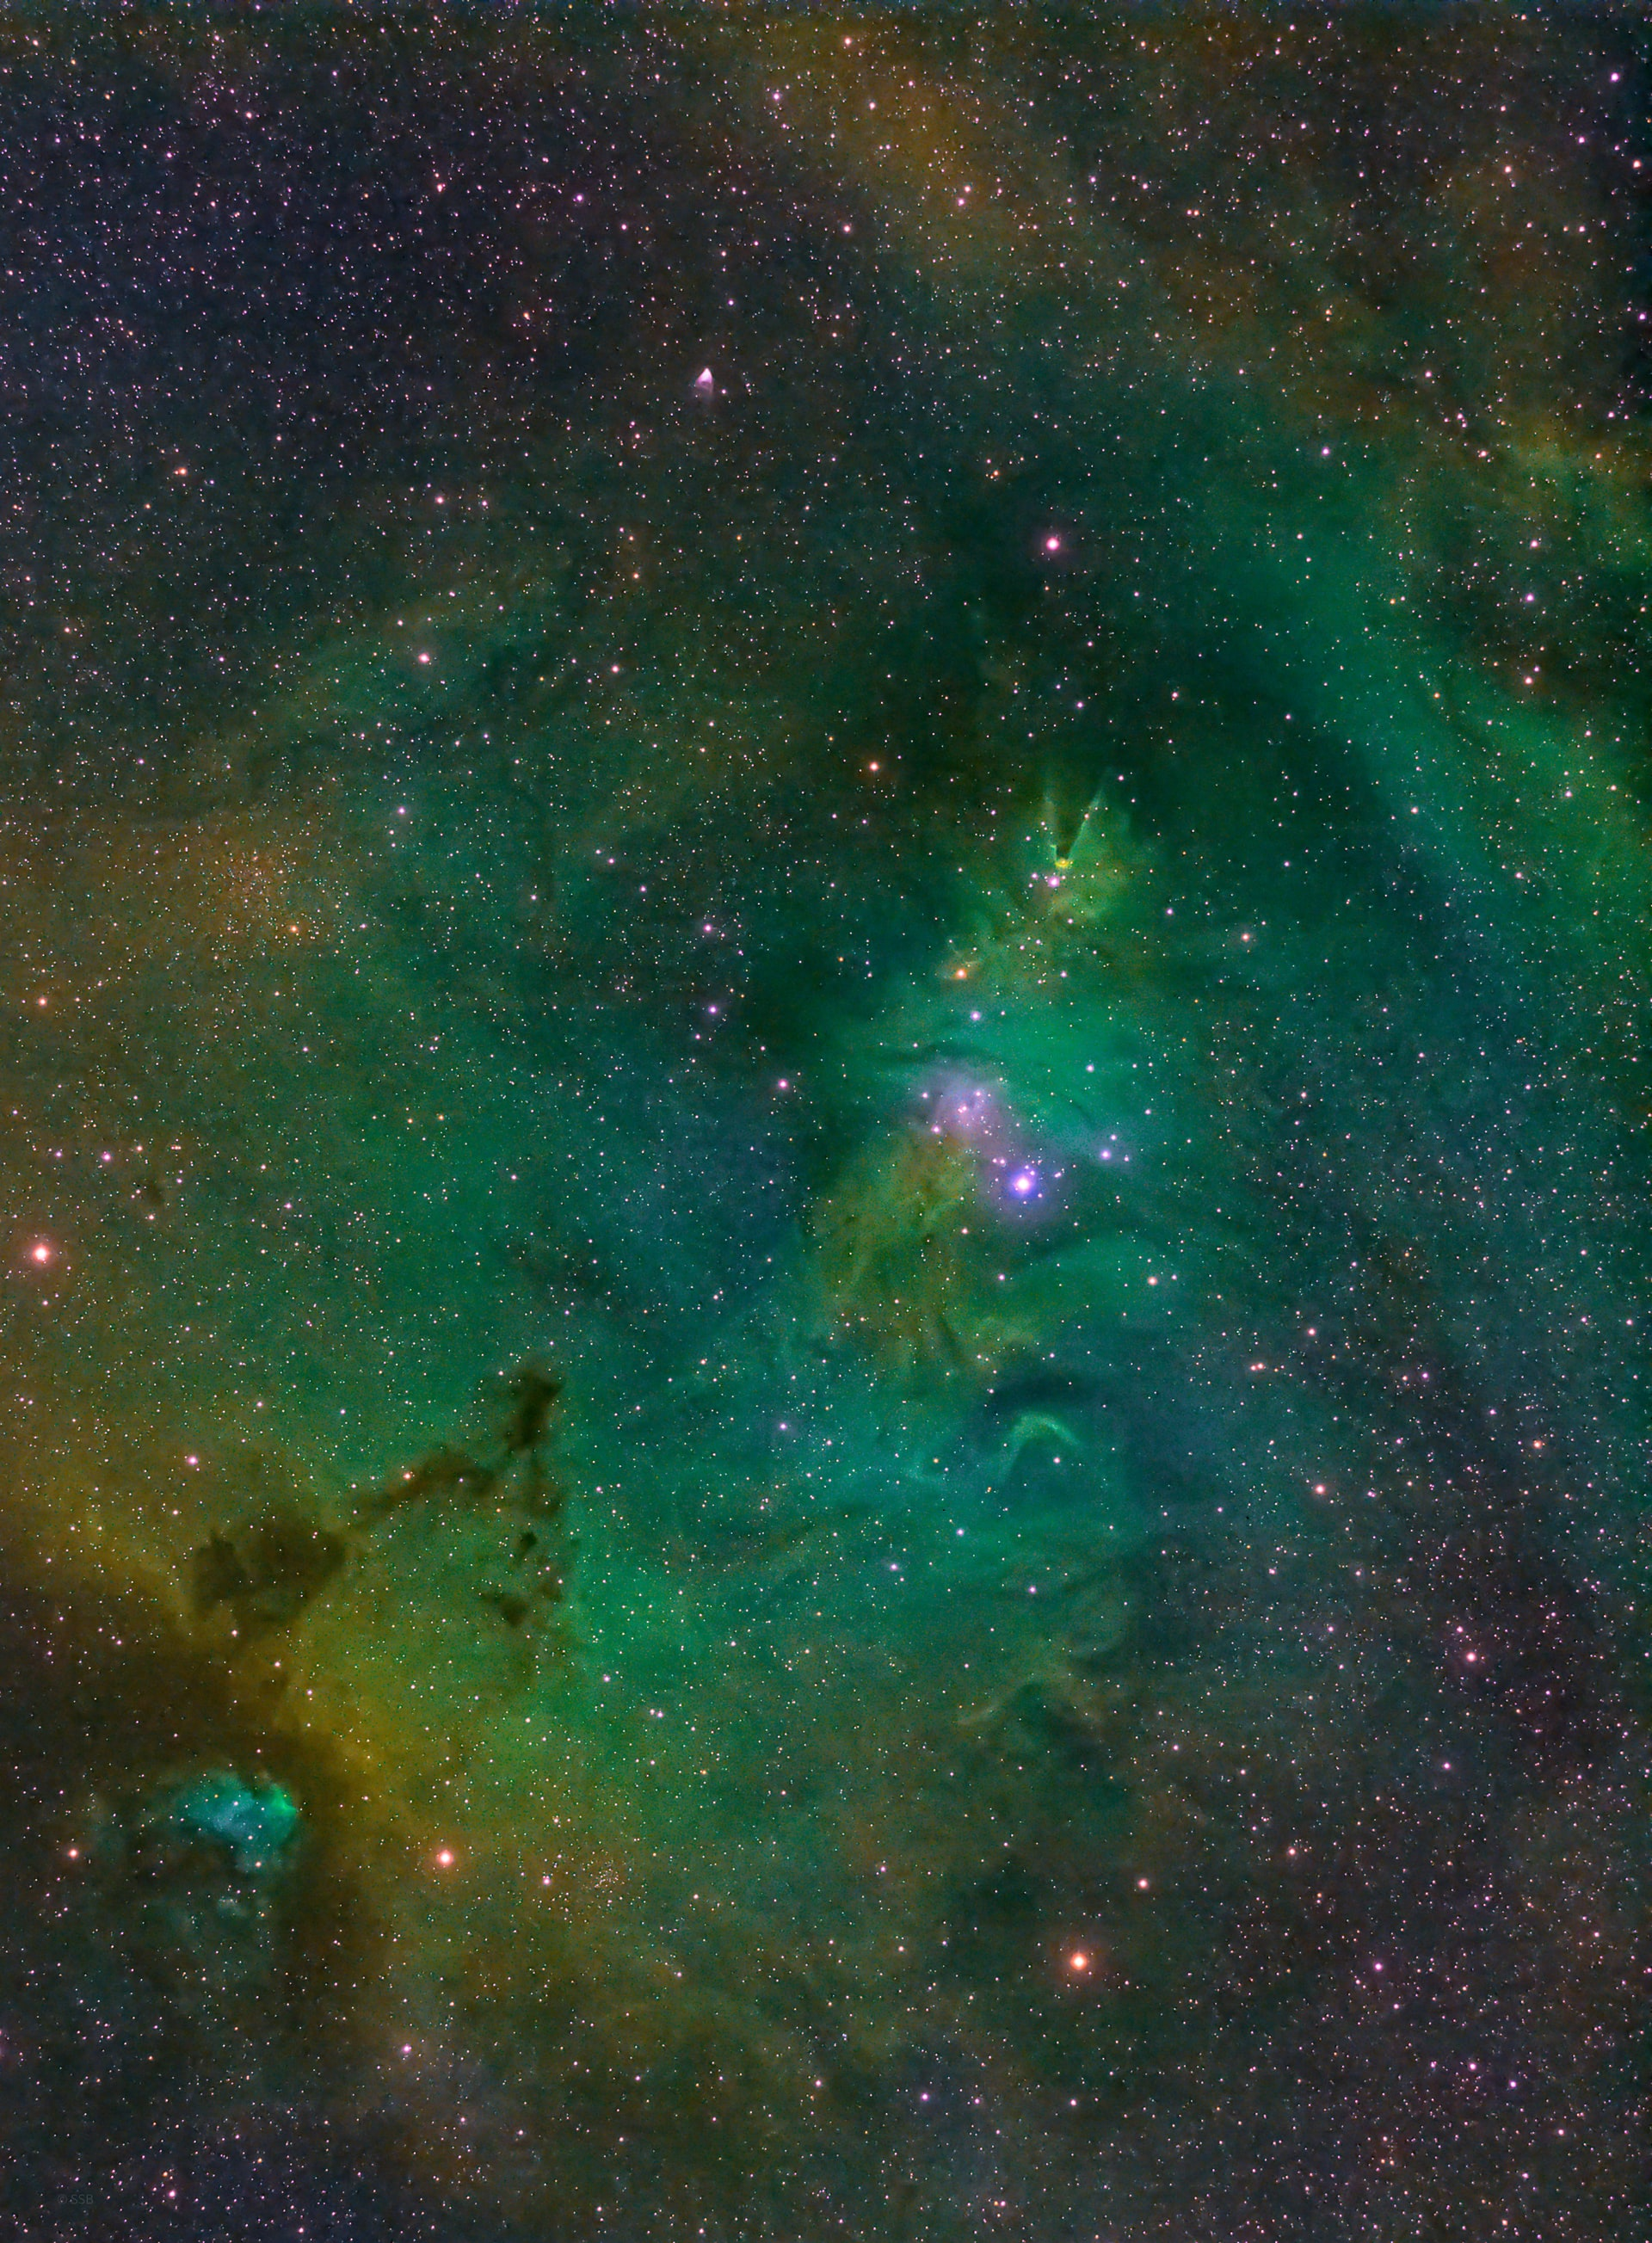
\includegraphics[width=\paperwidth]{./img/aldebaran.jpg}}
\begin{frame}
\huge{\textcolor{white}{\textbf{0xA: Architectural Attacks}}}
\end{frame}
}

\section{0xB: Attacks on the Web Server}
{
\usebackgroundtemplate{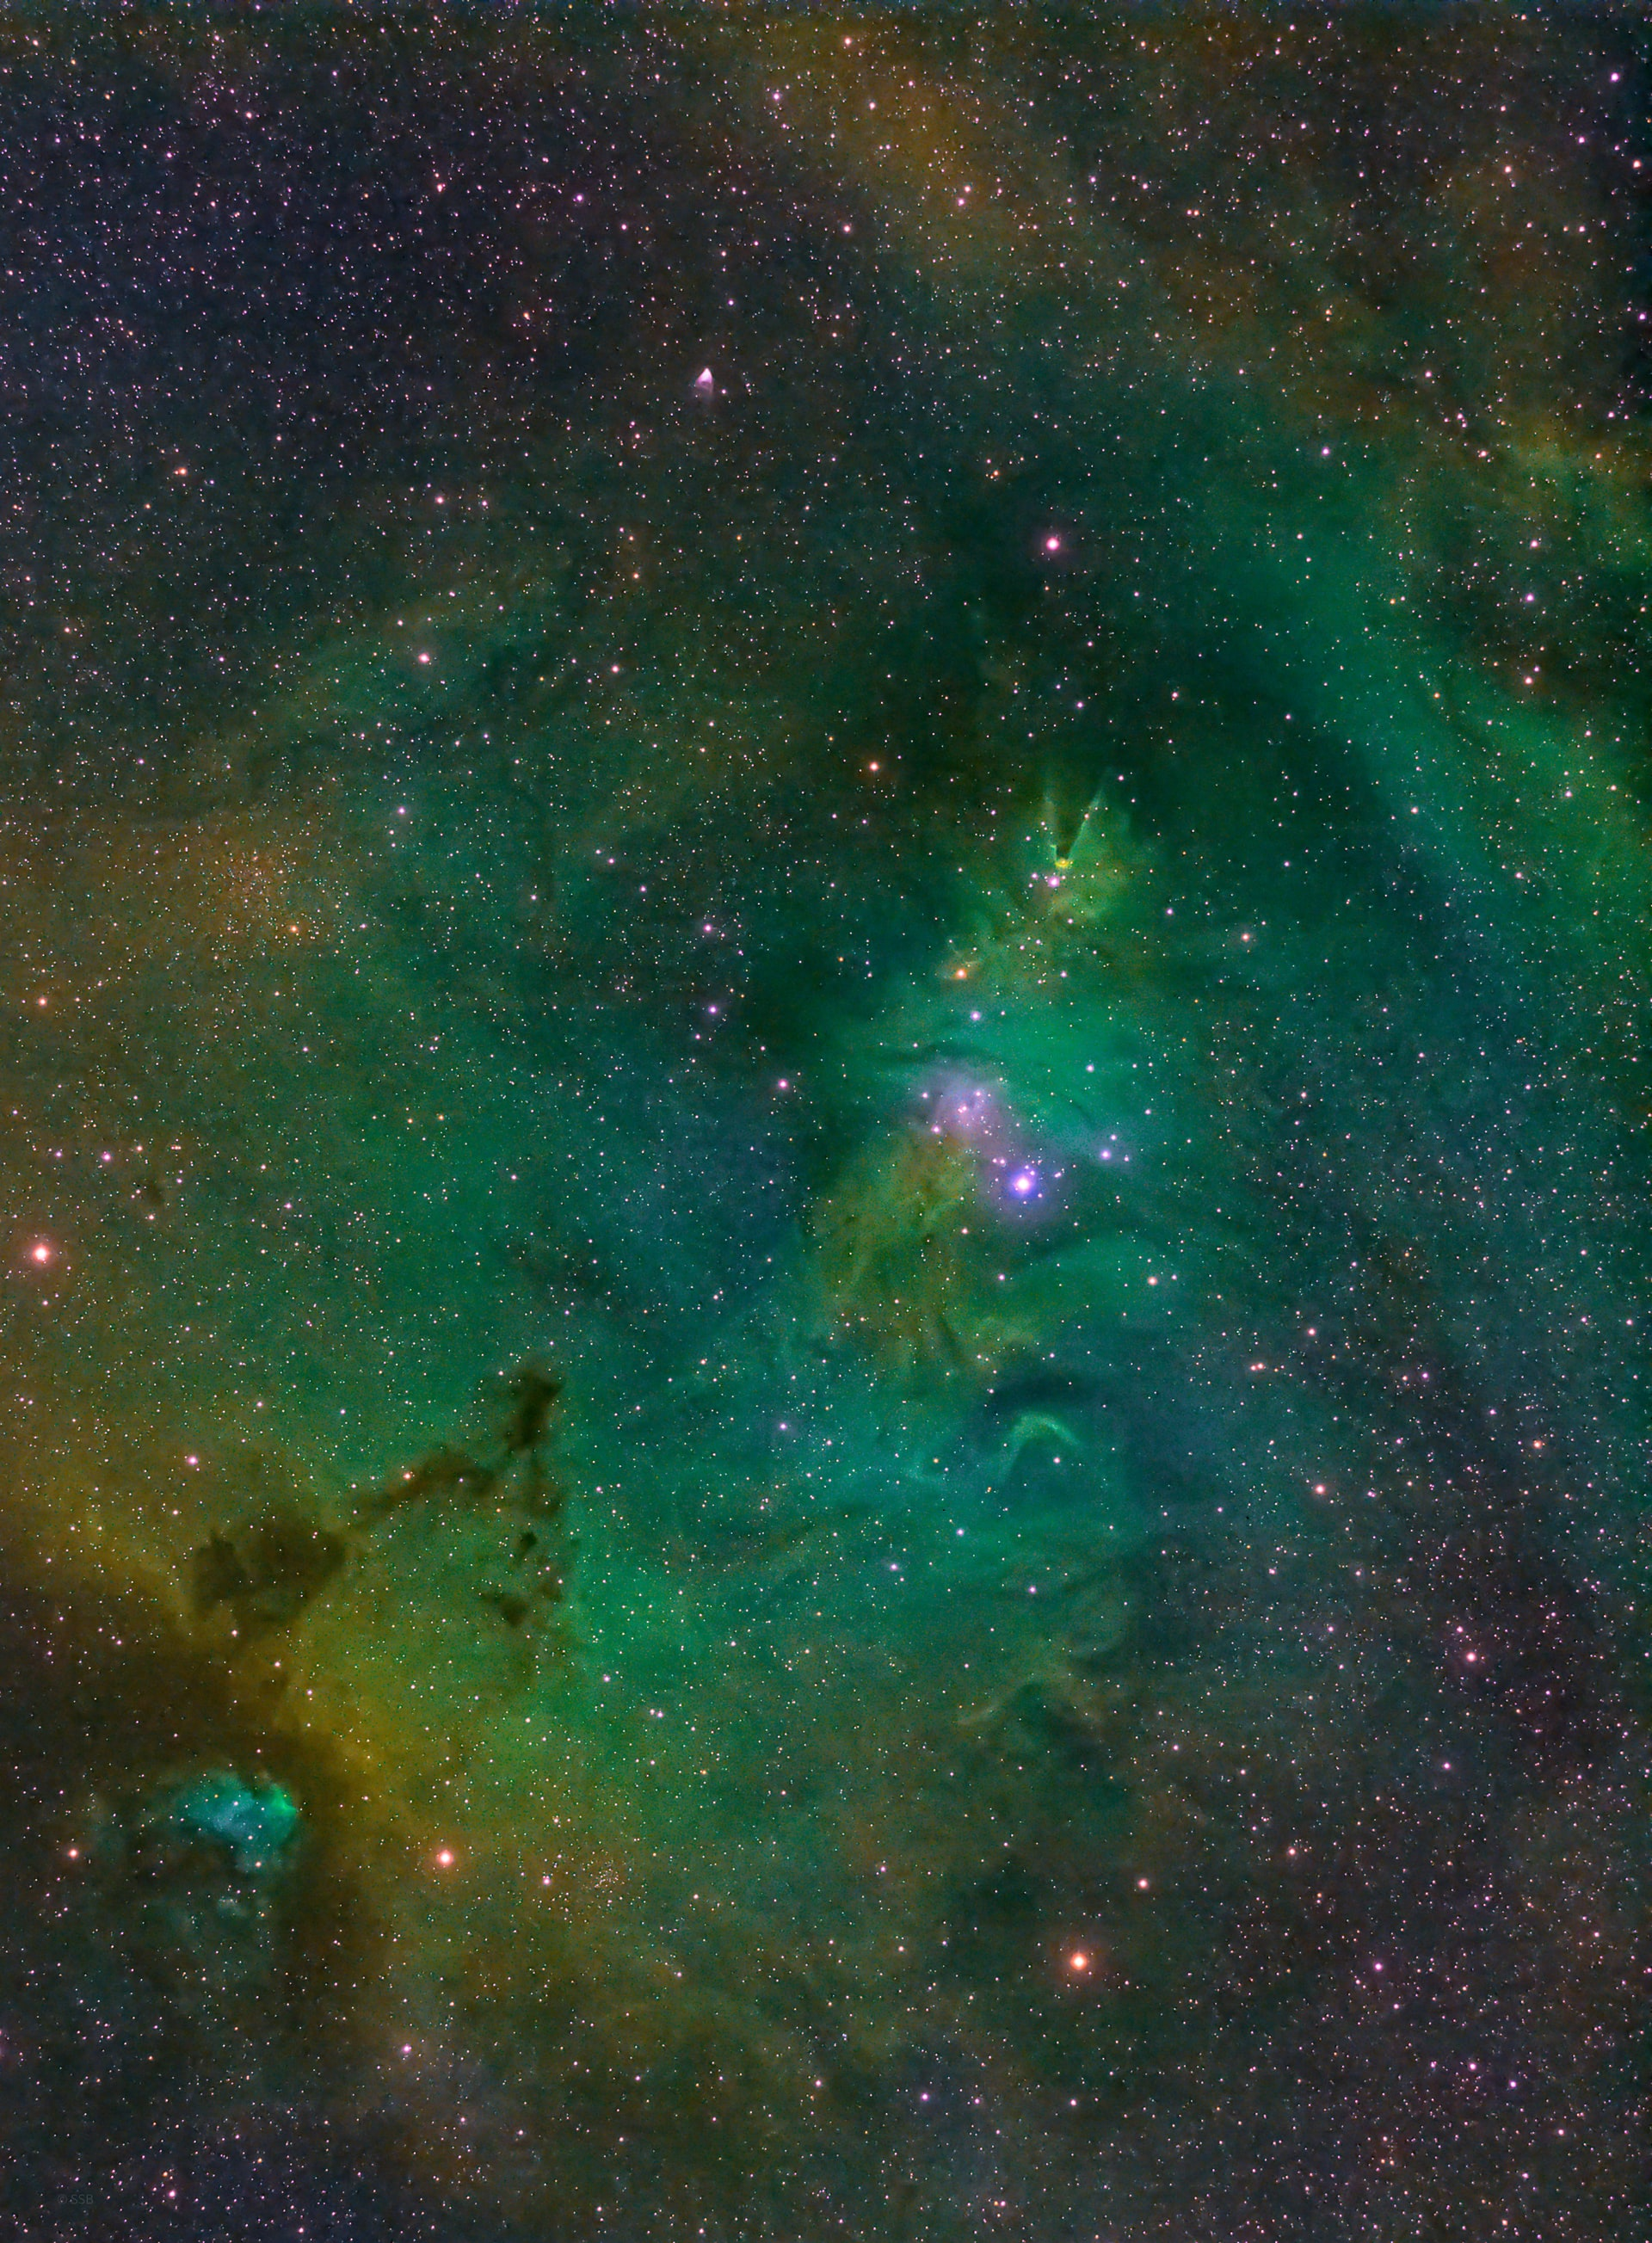
\includegraphics[width=\paperwidth]{./img/aldebaran.jpg}}
\begin{frame}
\huge{\textcolor{white}{\textbf{0xB: Attacks on the Web Server}}}
\end{frame}
}

\end{document}